
\chapter{壳模型\label{chap:=0058F3=006A21=00578B}}

\section{引言与普遍考虑\label{sec:=005F15=008A00=004E0E=00666E=00904D=008003=008651}}

在上一章中我们探讨了原子核的宏观整体性质，即全核或绝大部分核子协同参与的静态或动态集体行为。在这一章中，我们将讨论原子核完全不同的另一个重要物理层面：大量实验事实表明，核内的核子在很大程度上可以被视为在几乎未受扰动的单粒子轨道上独立运动的粒子。

正如我们在第 1 章开头指出的，独立粒子图像之所以在原子核这样强相互作用体系中成立，主要归因于 Pauli 不相容原理和量子力学测不准原理的深刻制约。现代核物理已经确立，现实核子-核子力在芯部（$c\simeq0.4\,\text{fm}$）处具有极强的硬芯排斥
\cite{Vi78}。因此，密堆积体积 $V_{c}$ 与原子核实际体积 $V$ 之比仅为 \cite{BM69}：

\begin{equation}
\frac{V_{c}}{V}=\left(\frac{c}{2r_{0}}\right)^{3}\simeq\frac{1}{100}\label{eq:packing_fraction}
\end{equation}

这意味着平均而言核子之间的距离相对较远，核子通常仅“感受”到核力吸引长程尾部。短程强排斥所诱发的剧烈硬碰撞由于 Pauli 原理对末态相空间的强烈冻结而极其罕见。由核散射实验估计的核内核子平均自由程至少与原子核自身线度相当
\cite{BM69,KK68}，这为核内独立粒子运动提供了最初步的坚实实验支撑。既然核子近似独立运动，这些单粒子运动必然受控于由所有其他核子共同产生的平均单体势阱中。

\section{壳效应的实验证据\label{sec:=0058F3=006548=005E94=007684=005B9E=009A8C=008BC1=00636E}}

核平均势的存在直接导致了类似于原子物理中电子壳层的特征能级聚集现象。实验上发现的核物理幻数（Magic numbers）：

\[
2,\;8,\;20,\;28,\;50,\;82,\;126
\]

构成了建立核壳模型最强有力的实验基石。在这些中子数或质子数处，原子核表现出异常强大的结合与极高的稳定性：
\begin{itemize}
\item 单粒子分离能：将最弱束缚核子从核中移走所需的能量定义为分离能 $S_{n}$ 或 $S_{p}$。图 2.1 表明，通常核的分离能约为
8 MeV，但在幻数处出现极为陡峭的骤降，双满壳核的分离能显著偏高，这一突变特征与原子稀有气体的电离能跃变完全类似；
\end{itemize}
\begin{figure}[H]
\begin{centering}
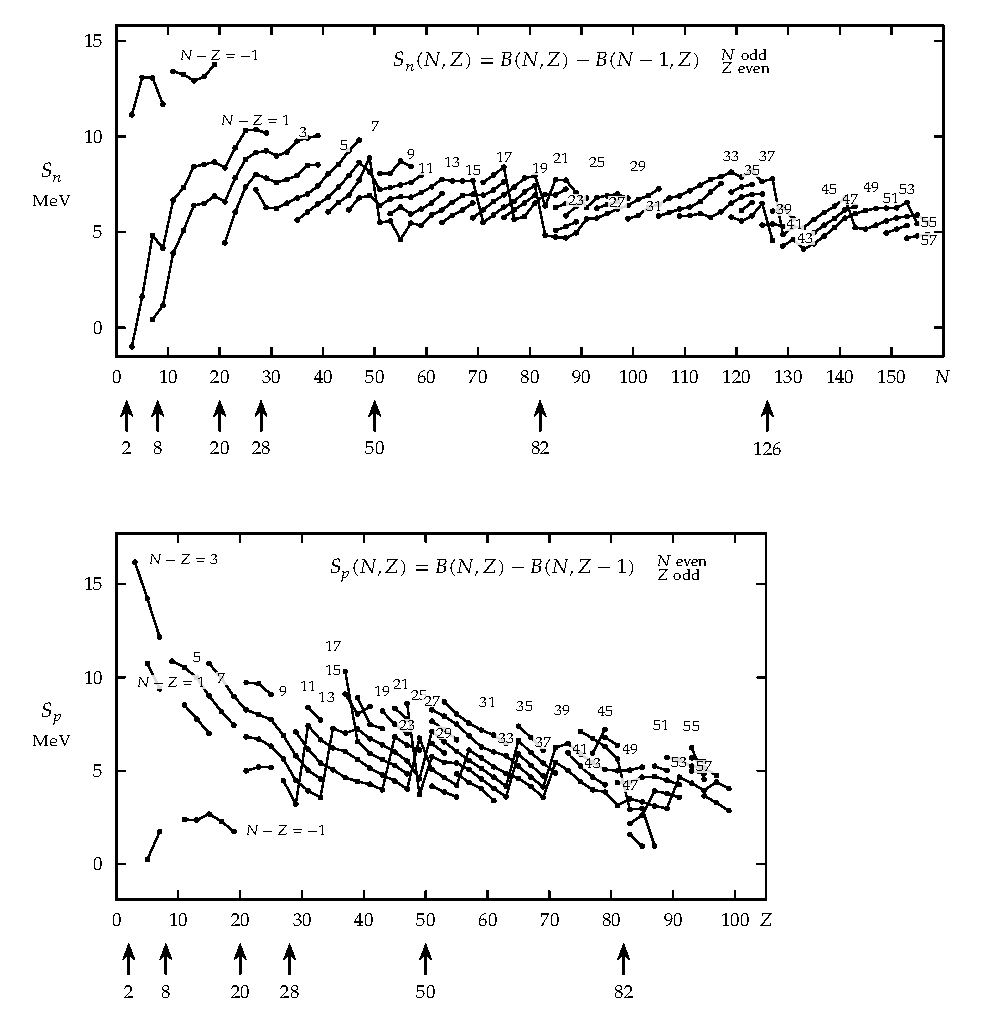
\includegraphics[width=0.75\textwidth]{pictures/2_1}
\par\end{centering}
\caption{\label{fig:2_1}图 2.1 中子与质子分离能分别作为中子数和质子数的函数（引自 {[}Ir 72{]}）。}
\end{figure}

\begin{itemize}
\item 质量与结合能偏差：实验核质量对 Bethe-Weizsäcker 半经验平滑质量公式的偏离（图 2.2）在幻数处呈现出极其显著的深下凹尖峰，表明幻数核具有异常强大的额外束缚能；
\end{itemize}
\begin{figure}[H]
\begin{centering}
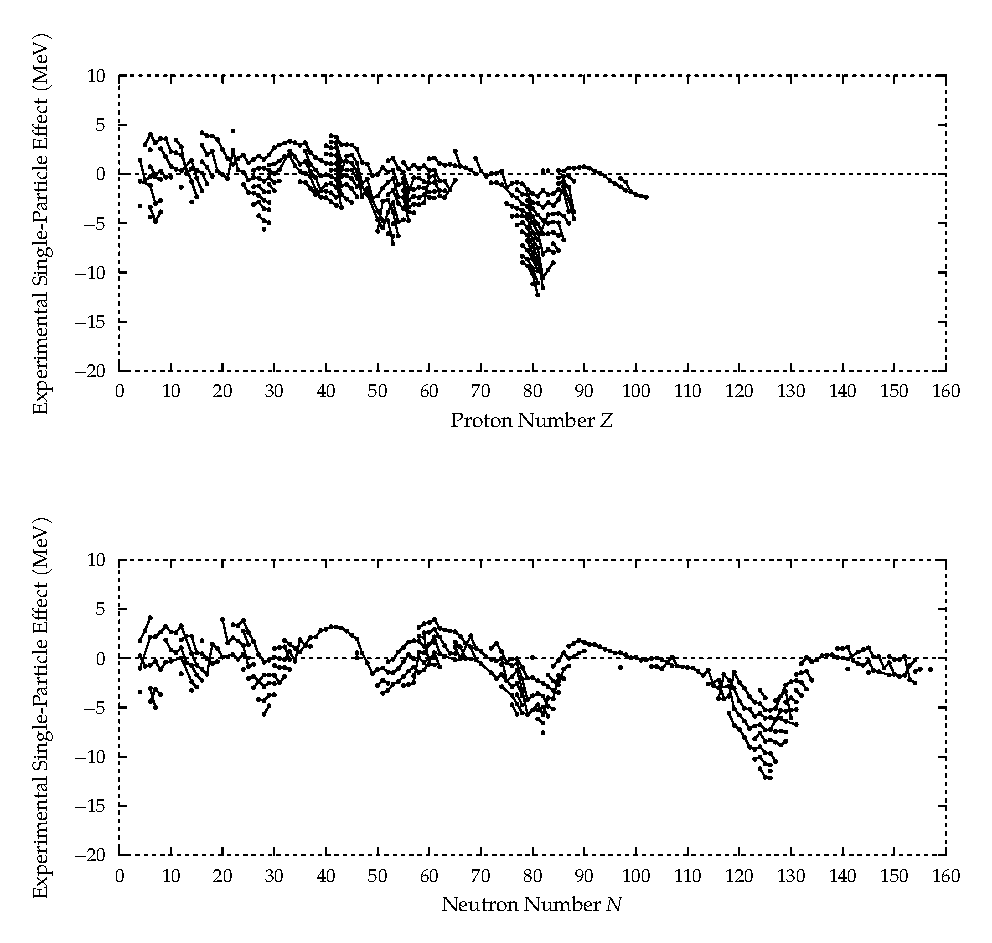
\includegraphics[width=0.75\textwidth]{pictures/2_2}
\par\end{centering}
\caption{\label{fig:2_2}图 2.2 实验核质量对平均平滑值的偏离作为中子数和质子数的函数（引自 {[}MS 66{]}）。}
\end{figure}

\begin{itemize}
\item 第一激发态能量与集体性：偶偶核的第一激发态 $2^{+}$ 能量在幻数闭壳处急剧升高（图 1.7），表明闭壳核对外场扰动具有极高的刚性，难以发生集体激发。
\end{itemize}

\section{原子核的平均势\label{sec:=00539F=005B50=006838=007684=005E73=005747=0052BF}}

在原子中，电子围绕带正电的原子核运动，天然存在一个外部提供的中心 Coulomb 场。而原子核内不存在任何外部中心场，其平均单体势阱是所有核子通过双体相互作用自洽形成的。在中心区域，核子受力均匀对称，净受力为零：

\begin{equation}
\left(\frac{\partial V}{\partial r}\right)_{r=0}=0\label{eq:pot_center_slope}
\end{equation}

随着离开核中心向核表面（$r=R_{0}$）过渡，束缚势阱逐渐变浅，$(\partial V/\partial r)_{r<R_{0}}>0$；在核外因强相互作用为短程力而迅速趋于零：$V(r)\to0$（$r\gg R_{0}$）。能够优美满足这些物理边界条件并与核电荷分布高度一致的唯象势是
Woods-Saxon 势 \cite{WS54}：

\begin{equation}
V_{\text{WS}}(r)=-V_{0}\left[1+\exp\left(\frac{r-R_{0}}{a}\right)\right]^{-1}\label{eq:woods_saxon_spherical}
\end{equation}

\begin{figure}[H]
\begin{centering}
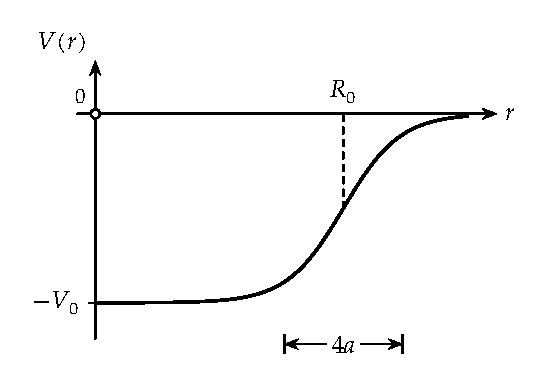
\includegraphics[width=0.75\textwidth]{pictures/2_3}
\par\end{centering}
\caption{\label{fig:2_3}图 2.3 Woods-Saxon 势的形式。}
\end{figure}

典型参数为势阱深度 $V_{0}\simeq50\,\text{MeV}$，核半径 $R_{0}=r_{0}A^{1/3}$（$r_{0}\simeq1.25\,\text{fm}$），表面弥散厚度参数
$a\simeq0.65\,\text{fm}$。为了解析讨论，物理上常采用两种极端势阱近似：
\begin{enumerate}
\item 各向同性谐振子势：$V(r)=-V_{0}+\frac{1}{2}m\omega^{2}_{0}r^{2}$；
\item 球方势阱：当 $r\leqslant R_{0}$ 时 $V(r)=-V_{0}$，当 $r>R_{0}$ 时 $V(r)=0$（或考虑无穷深球方势阱）。
\end{enumerate}
对于三维球形谐振子，能级为等间距能级：

\begin{equation}
\varepsilon_{N}=\hbar\omega_{0}\left(N+\frac{3}{2}\right)-V_{0},\quad N=2(n-1)+l\label{eq:ho_spectrum_spherical}
\end{equation}

其中主量子数 $N=0,1,2,\dots$，径向量子数 $n=1,2,\dots$，轨道角动量 $l=0,1,\dots,N$
与 $N$ 具有相同的奇偶性（同一振子壳层只包含相同宇称态）。考虑自旋后，每个主振子壳层的简并度为：

\begin{equation}
D(N)=(N+1)(N+2)\label{eq:ho_degeneracy}
\end{equation}

谐振子频率 $\hbar\omega_{0}$ 可由核电荷均方半径与核饱和密度确定 \cite{Mo57}：

\begin{equation}
\hbar\omega_{0}\simeq\frac{5}{4}\left(\frac{3}{2}\right)^{1/3}\frac{\hbar^{2}}{mr^{2}_{0}}A^{-1/3}\simeq41\cdot A^{-1/3}\,\text{[MeV]}\label{eq:period_of_shell}
\end{equation}

振子特征长度为 $b=\sqrt{\hbar/(m\omega_{0})}\simeq1.01\cdot A^{1/6}\,\text{[fm]}$。谐振子势填满主壳层的累积核子数为：2,
8, 20, 40, 70, 112, 168。在更真实的方势阱或 Woods-Saxon 势中，由于势阱边界比谐振子势更陡峭，高
$l$ 轨道的能量显著降低，从而消除了谐振子势中的偶然简并，给出能级序列：$1s,1p,1d,2s,1f,2p,1g,\dots$，对应的壳闭合幻数为
2, 8, 20, 34, 40, 58, 92, 138。显然，无论是谐振子势还是球方势阱，都只能解释前三个幻数（2, 8, 20），而完全无法给出重核区正确的实验幻数
28, 50, 82, 126。

\begin{figure}[H]
\begin{centering}
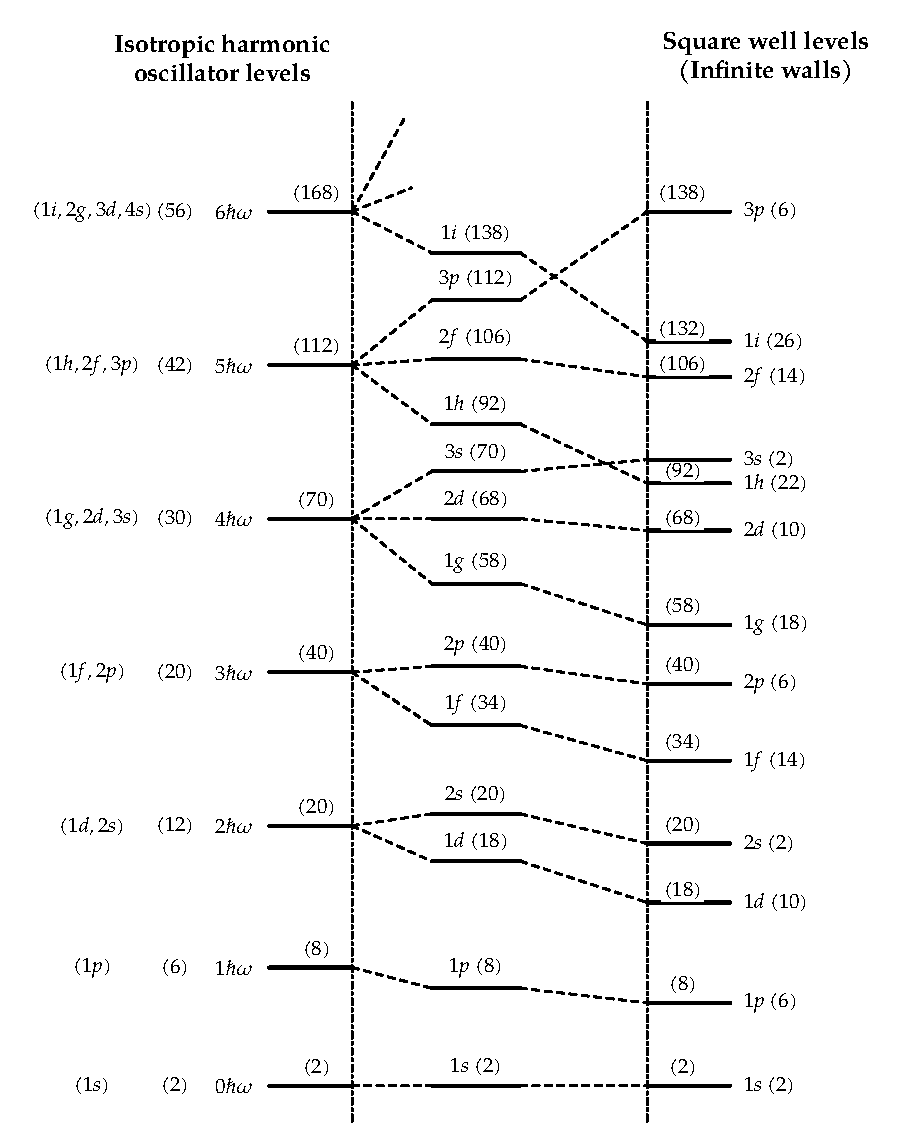
\includegraphics[width=0.75\textwidth]{pictures/2_4}
\par\end{centering}
\caption{\label{fig:2_4}图 2.4 各向同性谐振子（左）与无限深球方势阱（右）的单粒子能级方案（引自 {[}MJ 55{]}）。}
\end{figure}


\section{自旋-轨道耦合\label{sec:=0081EA=0065CB-=008F68=009053=008026=005408}}

1949 年，Mayer \cite{Ma49} 与 Haxel、Jensen、Suess \cite{HJS49} 独立提出，解决这一重大难题的关键在于核单粒子势中存在强大的自旋-轨道相互作用：

\begin{equation}
V_{ls}(\boldsymbol{r})=V_{ls}(r)\boldsymbol{l}\cdot\boldsymbol{s}=\kappa\frac{1}{r}\frac{\mathrm{d}V(r)}{\mathrm{d}r}\,\boldsymbol{l}\cdot\boldsymbol{s}\label{eq:spin_orbit_potential}
\end{equation}

与原子中由相对论 Thomas 进动引起的微弱自旋-轨道耦合不同，核物理中的自旋-轨道力强度不仅比原子大近 30 倍，而且符号相反（$\kappa<0$）。核子的总单粒子角动量为
$\boldsymbol{j}=\boldsymbol{l}+\boldsymbol{s}$，由 $\boldsymbol{l}\cdot\boldsymbol{s}=\frac{1}{2}(\boldsymbol{j}^{2}-\boldsymbol{l}^{2}-\boldsymbol{s}^{2})$
可得算符本征值为：

\begin{equation}
\langle\boldsymbol{l}\cdot\boldsymbol{s}\rangle=\begin{cases}
\frac{1}{2}l, & \text{对于 }j=l+\frac{1}{2}\\
-\frac{1}{2}(l+1), & \text{对于 }j=l-\frac{1}{2}
\end{cases}\label{eq:ls_eigenvalues}
\end{equation}

由此导致的同一 $l$ 轨道的能级分裂量为：

\begin{equation}
\Delta\varepsilon_{ls}=\varepsilon_{j=l-1/2}-\varepsilon_{j=l+1/2}=\left(l+\frac{1}{2}\right)\langle V_{ls}\rangle\label{eq:ls_splitting}
\end{equation}

由于 $V_{ls}(r)$ 为强吸引作用，平行耦合的轨道（$j=l+1/2$）能量大幅度下移，而反平行轨道（$j=l-1/2$）能量上移。分裂量正比于
$2l+1$，随轨道角动量 $l$ 急剧增大！在每个主要高能壳层中，具有最高角动量的支能级：
\begin{itemize}
\item $1f_{7/2}$（来自 $N=3$ 壳）被强力压低，在 20 之后容纳 8 个核子，形成幻数 $\mathbf{28}$；
\item $1g_{9/2}$（来自 $N=4$ 壳）侵入下一壳层，在 40 之后容纳 10 个核子，形成幻数 $\mathbf{50}$；
\item $1h_{11/2}$（来自 $N=5$ 壳）侵入形成幻数 $\mathbf{82}$；
\item $1i_{13/2}$（来自 $N=6$ 壳）侵入形成幻数 $\mathbf{126}$。
\end{itemize}
这些被强自旋-轨道耦合压入低主振子壳层的高角动量轨道被称为侵入态（Intruder states）。它们与其所在壳层中的其他轨道具有相反的宇称，因而在单核子衰变中受到宇称选择定则的强力保护。由此，包含强自旋-轨道相互作用的球形单粒子壳模型彻底、自然地解释了全核素区的全部幻数（图
2.5）！

\begin{figure}[H]
\begin{centering}
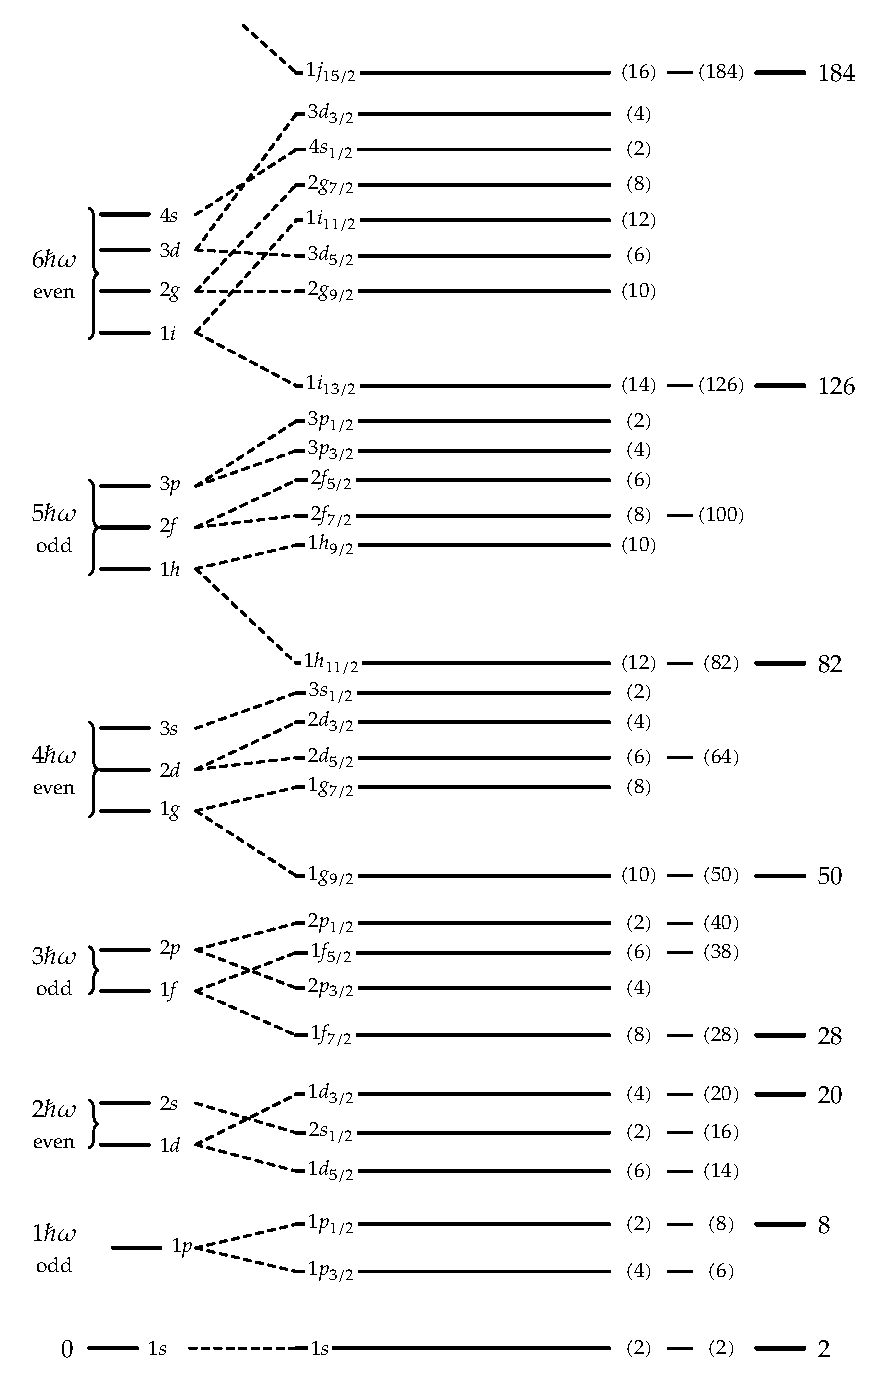
\includegraphics[width=0.75\textwidth]{pictures/2_5}
\par\end{centering}
\caption{\label{fig:2_5}图 2.5 包含自旋-轨道耦合项的壳模型核能级示意图（引自 {[}MJ 55{]}）。}
\end{figure}


\section{多体问题的壳模型方法\label{sec:=00591A=004F53=0095EE=009898=007684=0058F3=006A21=00578B=0065B9=006CD5}}

严格的原子核微观理论建立在非相对论量子多体问题之上，其总微观 Hamilton 量包含核子动能与两体相互作用：

\begin{equation}
H=\sum^{A}_{i=1}t_{i}+\frac{1}{2}\sum^{A}_{i\neq j}v(i,j)\label{eq:full_microscopic_H}
\end{equation}

其中 $i=(\boldsymbol{r}_{i},\boldsymbol{s}_{i},\boldsymbol{t}_{i})$
表示单个核子的全部空间、自旋与同位旋坐标。壳模型方法的核心思想是在总 Hamilton 量中引入一个平均单粒子势场 $U(i)$，并将全
Hamilton 量精确分解为无相互作用的独立粒子单体 Hamilton 量 $H_{0}$ 与剩余相互作用（Residual interaction）$V_{\text{res}}$：

\begin{equation}
H=H_{0}+V_{\text{res}}\label{eq:H_split_H0_Vres}
\end{equation}

其中：

\begin{align}
H_{0} & =\sum^{A}_{i=1}h(i)=\sum^{A}_{i=1}\left[t_{i}+U(i)\right]\nonumber \\
V_{\text{res}} & =\frac{1}{2}\sum^{A}_{i\neq j}v(i,j)-\sum^{A}_{i=1}U(i)\label{eq:V_residual_def}
\end{align}

求解单粒子薛定谔方程：

\begin{equation}
h(i)\phi_{k}(i)=\varepsilon_{k}\phi_{k}(i)\label{eq:single_particle_schrodinger}
\end{equation}

本征态 $\phi_{k}$ 构成二次量子化表象（附录 C）的正交归一基底。设 $a^{\dagger}_{k}$ 与 $a_{k}$
分别为轨道 $k$ 上的费米子产生与湮灭算符，则独立粒子 Hamilton 量可写为：

\begin{equation}
H_{0}=\sum_{k}\varepsilon_{k}a^{\dagger}_{k}a_{k}\label{eq:H0_second_quantized}
\end{equation}

对于双满壳闭壳核，核子从最低轨道一直填到 Fermi 能级 $\varepsilon_{F}$，体系基态由单一 Slater 行列式给出：

\begin{equation}
|\Phi_{0}\rangle=\prod_{i\leqslant\varepsilon_{F}}a^{\dagger}_{i}|-\rangle\label{eq:slater_ground_state}
\end{equation}

\begin{figure}[H]
\begin{centering}
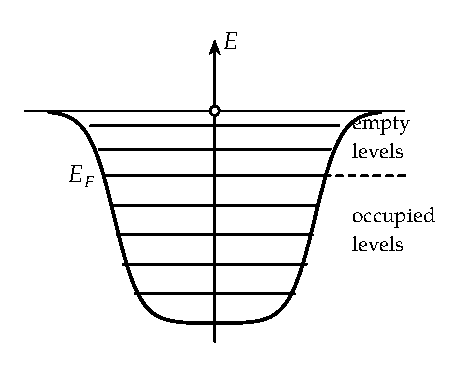
\includegraphics[width=0.75\textwidth]{pictures/2_6}
\par\end{centering}
\caption{\label{fig:2_6}图 2.6 壳模型势阱与费米能级示意图。}
\end{figure}

对于中子过剩核，由于质子感受到额外的 Coulomb 排斥能，其势能曲面整体上移；同时核对称能使质子感受到的核势部分比中子势更深，从而使中子与质子的
Fermi 面得以保持平衡（图 2.7）。

\begin{figure}[H]
\begin{centering}
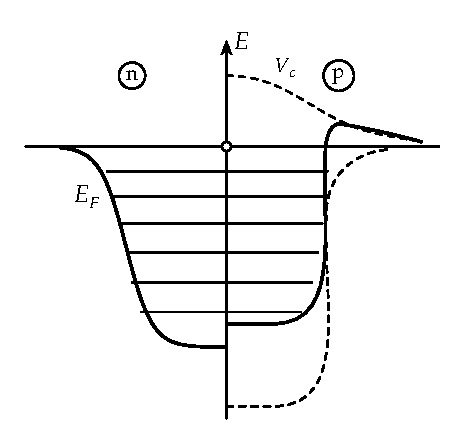
\includegraphics[width=0.75\textwidth]{pictures/2_7}
\par\end{centering}
\caption{\label{fig:2_7}图 2.7 中子过剩核中中子与质子壳模型势的比较（虚线对应更深的质子核势部分）。}
\end{figure}

在 Fermi 气体图像下，体系最简单的激发态是将 Fermi 海中的一个核子 $i$（$\varepsilon_{i}\leqslant\varepsilon_{F}$）激发到空轨道
$m$（$\varepsilon_{m}>\varepsilon_{F}$）上，形成粒子-空穴激发态（$1p-1h$ 态）：

\begin{equation}
|\Phi_{mi}\rangle=a^{\dagger}_{m}a_{i}|\Phi_{0}\rangle,\quad\Delta E_{mi}=\varepsilon_{m}-\varepsilon_{i}\label{eq:ph_excitation}
\end{equation}

\begin{figure}[H]
\begin{centering}
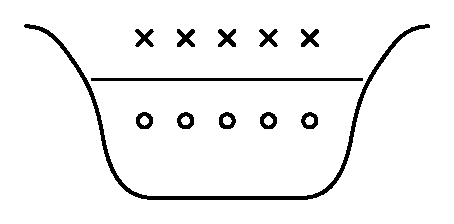
\includegraphics[width=0.75\textwidth]{pictures/2_8}
\par\end{centering}
\caption{\label{fig:2_8}图 2.8 典型的五粒子（叉号）五空穴（空心圆）激发态示意图。}
\end{figure}

极其便利的工具是定义准粒子（Quasiparticles）：

\begin{equation}
\alpha^{\dagger}_{m}=a^{\dagger}_{m}\;(\varepsilon_{m}>\varepsilon_{F}),\quad\alpha^{\dagger}_{i}=a_{i}\;(\varepsilon_{i}\leqslant\varepsilon_{F})\label{eq:quasiparticle_particle_hole}
\end{equation}

使得基态成为准粒子真空态：$\alpha_{k}|\Phi_{0}\rangle=0$。真实的核基态由于剩余相互作用 $V_{\text{res}}$
的存在，包含着虚粒子-空穴激发的相关混杂：

\begin{equation}
|\Psi\rangle=c_{0}|\Phi_{0}\rangle+\sum_{mi}c_{mi}a^{\dagger}_{m}a_{i}|\Phi_{0}\rangle+\frac{1}{4}\sum_{mnij}c_{mnij}a^{\dagger}_{m}a^{\dagger}_{n}a_{j}a_{i}|\Phi_{0}\rangle+\dots\label{eq:ground_state_correlation_expansion}
\end{equation}

在良好的平均场势阱下，展开系数满足 $c_{0}\approx1$，高阶关联较小。如何在微观上自洽决定最优平均势 $U(i)$
使得剩余相互作用最小，正是第 5 章 Hartree-Fock 理论的核心议题。

\section{对称性\label{sec:=005BF9=0079F0=006027}}

\subsection{平移对称性}

真实的原子核 Hamilton 量在全空间中具有严格的平移不变性。然而在唯象壳模型中，为了定义单粒子势场，我们人为地将平均势的中心固定在空间原点，这必然破坏了平移对称性。这种对称性破缺带来的最直接后果是：体系的激发能谱中混入了多余的自由度，产生所谓的赝态或赝模（Spurious
states / Spurious modes）。

由于一个包含 $A$ 个核子的体系只有 $3A-3$ 个内秉自由度，壳模型的 $3A$ 个坐标中包含了核质心整体在势阱中的振荡运动。在谐振子势中，总
Hamilton 量可以精确分离为质心部分与相对运动部分：

\begin{equation}
H=H_{\text{c.m.}}+H_{\text{rel}}=\left(\frac{\boldsymbol{P}^{2}}{2mA}+\frac{1}{2}mA\omega^{2}_{0}\boldsymbol{R}^{2}\right)+H_{\text{rel}}\label{eq:trans_cm_separation}
\end{equation}

其中 $\boldsymbol{R}=\frac{1}{A}\sum_{i}\boldsymbol{r}_{i}$，$\boldsymbol{P}=\sum_{i}\boldsymbol{p}_{i}$。因此质心零点能为
$\frac{3}{2}\hbar\omega_{0}$。为了消除赝质心动能带来的误差，通常从总能量中减去质心动能期望值 $\langle\boldsymbol{P}^{2}\rangle/(2mA)$；在第
11 章中我们将系统讨论通过投影算符方法严格消除平移赝态的微观理论。

\subsection{转动对称性与组态混合}

球形壳模型 Hamilton 量 $H_{0}$（包含自旋-轨道耦合项）与总角动量算符 $\boldsymbol{J}^{2}$
及 $J_{z}$ 对易：

\begin{equation}
\boldsymbol{J}=\sum^{A}_{i=1}\boldsymbol{j}_{i},\quad J_{z}=\sum^{A}_{i=1}j_{zi}\label{eq:total_J_def}
\end{equation}

对于双满壳闭壳核，所有单粒子态全部被填满，基态唯一的总角动量本征值严格为 $I=0^{+}$，该结论已被所有双幻核无一例外地实验证实。当闭壳核外只有一个核子（或缺少一个核子形成的单空穴态）时，核基态总角动量自然等于该价核子的单粒子角动量
$I=j$。

当闭壳核外存在两个以上价核子时，同一 $j$ 壳层内不同磁量子数 $m$ 的状态是完全简并的。例如对于同种价核子组态 $(j)^{2}$，根据角动量耦合理论与
Clebsch-Gordan 系数：

\begin{equation}
|IM\rangle=\frac{1}{\sqrt{2}}\sum_{m_{1}m_{2}}C^{IM}_{jm_{1}jm_{2}}|m_{1}m_{2}\rangle\label{eq:cg_two_particle_coupling}
\end{equation}

由于核子是全同费米子，双粒子态满足反对称性 $|m_{2}m_{1}\rangle=-|m_{1}m_{2}\rangle$，结合
Clebsch-Gordan 系数的对称性性质 $C^{IM}_{jm_{2}jm_{1}}=(-1)^{2j-I}C^{IM}_{jm_{1}jm_{2}}$，得到波函数具有因子
$1-(-1)^{2j-I}=1+(-1)^{I}$（因为对半整数 $j$，$2j$ 为奇数）。因此非零的物理态要求总角动量必须为偶数：

\begin{equation}
I=0,2,4,\dots,2j-1\label{eq:even_I_allowed}
\end{equation}

例如对于 $j=3/2$，允许的总角动量仅为 $I=0,2$。为了在这些简并态中确定基态能量并解除简并，必须引入剩余相互作用 $V_{\text{res}}$（式
(2.35)）并在模型组态空间中进行对角化。在真实的核中，配对相互作用使得 $I=0$ 态的能量显著降低，从而在理论上保证了所有偶偶核基态自旋恒为
$0^{+}$。

对于远离闭壳的核，单组态壳模型常常失效，必须考虑组态混合（Configuration mixing）：即真实的核本征态是不同粒子-空穴组态和不同单粒子轨道
Slater 行列式的相干叠加：

\begin{equation}
|\Psi_{I}\rangle=\sum_{\alpha}c_{\alpha}|\Phi_{\alpha}(I)\rangle\label{eq:config_mixing_wavefunction}
\end{equation}

组态混合不仅解除了开壳层能级的简并，而且是微观核结构中产生集体相干性与核形变的核心机制。

\subsection{同位旋}

核力强烈的电荷无关性（Charge independence，见第 4 章）表明，除微弱的电磁相互作用外，质子和中子在强核力作用下表现出高度的一致性。Heisenberg
\cite{He32} 与 Wigner \cite{Wi37} 由此引入了同位旋（Isotopic spin / Isospin）概念，将质子与中子视为同一种粒子——核子（Nucleon）的两个不同内秉荷电状态。

单个核子的同位旋算符由 Pauli 矩阵表示：$\boldsymbol{t}=\frac{1}{2}\boldsymbol{\tau}$，其基矢为：

\begin{equation}
|p\rangle=\begin{pmatrix}1\\
0
\end{pmatrix},\quad|n\rangle=\begin{pmatrix}0\\
1
\end{pmatrix}\label{eq:isospin_spinors}
\end{equation}

在核物理的传统约定中，$t_{3}$ 的本征值为：

\begin{equation}
t_{3}|n\rangle=\frac{1}{2}|n\rangle,\quad t_{3}|p\rangle=-\frac{1}{2}|p\rangle\label{eq:isospin_t3_eigenvals}
\end{equation}

升降算符 $t_{\pm}=t_{1}\pm\mathrm{i}t_{2}$ 实现质子与中子状态的相互跃迁：$t_{-}|n\rangle=|p\rangle$，$t_{+}|p\rangle=|n\rangle$。对于包含
$A$ 个核子的体系，总同位旋矢量算符定义为：

\begin{equation}
\boldsymbol{T}=\sum^{A}_{i=1}\boldsymbol{t}_{i},\quad T_{3}=\sum^{A}_{i=1}t_{3i}=\frac{1}{2}(N-Z)\label{eq:total_isospin_def}
\end{equation}

若忽略 Coulomb 力，总 Hamilton 量与 $\boldsymbol{T}^{2}$ 和 $T_{3}$ 对易，体系的每个定态都具有良好的总同位旋量子数
$T$（满足 $T\geqslant|T_{3}|$）。例如对于质量数 $A=10$ 的同量异位素三胞胎 $\ce{^{10}Be}$（$T_{3}=1$）、$\ce{^{10}B}$（$T_{3}=0$）与
$\ce{^{10}C}$（$T_{3}=-1$），存在严格对应的同位旋三重态（$T=1$，图 2.9）；此外 $\ce{^{10}B}$
独有 $T=0$ 的单态。

\begin{figure}[H]
\begin{centering}
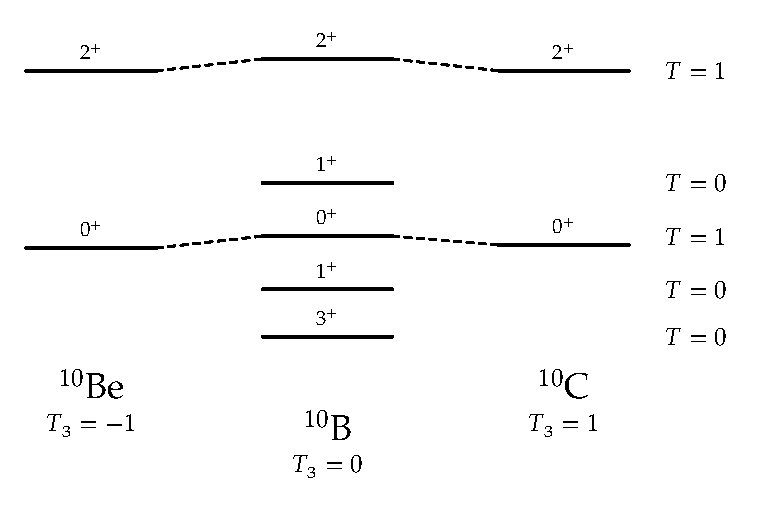
\includegraphics[width=0.75\textwidth]{pictures/2_9}
\par\end{centering}
\caption{\label{fig:2_9}图 2.9 同量异位素激发谱中的同位旋三重态与单态（引自 {[}MJ 55{]}）。}
\end{figure}

由同位旋上升算符 $T_{+}$ 作用在满壳组态上为零可知，所有占据质子能级同时被中子占据的壳模型态必有 $T=T_{3}=(N-Z)/2$，基态组态如图
2.10 所示。

\begin{figure}[H]
\begin{centering}
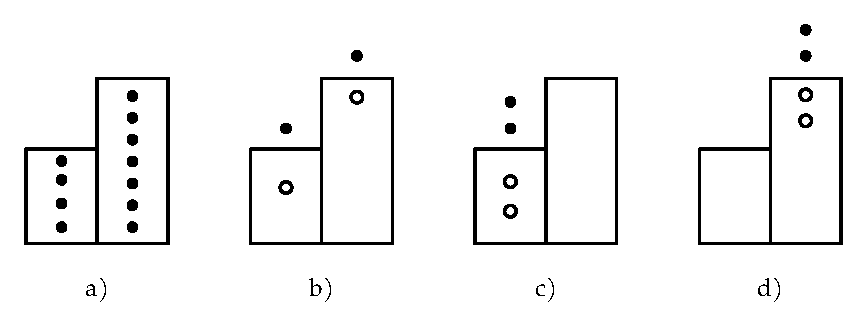
\includegraphics[width=0.75\textwidth]{pictures/2_10}
\par\end{centering}
\caption{\label{fig:2_10}图 2.10 壳模型组态与同位旋示意图。}
\end{figure}

在重核中，虽然质子间巨大的 Coulomb 排斥能破坏了严格的同位旋守恒，但由于大量过剩中子形成了强同位旋矢量单粒子势垒（Symmetry
potential），阻碍了不同同位旋组态的混杂，使得重核低激发态仍然保持着高度纯净的同位旋，并在核反应中观察到了极其清晰锐利的同位旋类似态（Isobaric
Analogue States, IAS）。

\section{与实验对比\label{sec:=004E0E=005B9E=009A8C=005BF9=006BD4}}

\subsection{单粒子（空穴）态的实验证据}

单粒子壳模型最直接的实验检验是在双闭壳核附近的单核子转移反应与敲出反应：
\begin{itemize}
\item 条带反应与单核子拾取：如 $(d,p)$、$(p,d)$、$(d,t)$ 反应，通过测量转移出射粒子的角分布和截面，能够直接提取残核能级的轨道角动量
$l$ 与光谱学因子（Spectroscopic factor）$S_{j}$；
\end{itemize}
\begin{figure}[H]
\begin{centering}
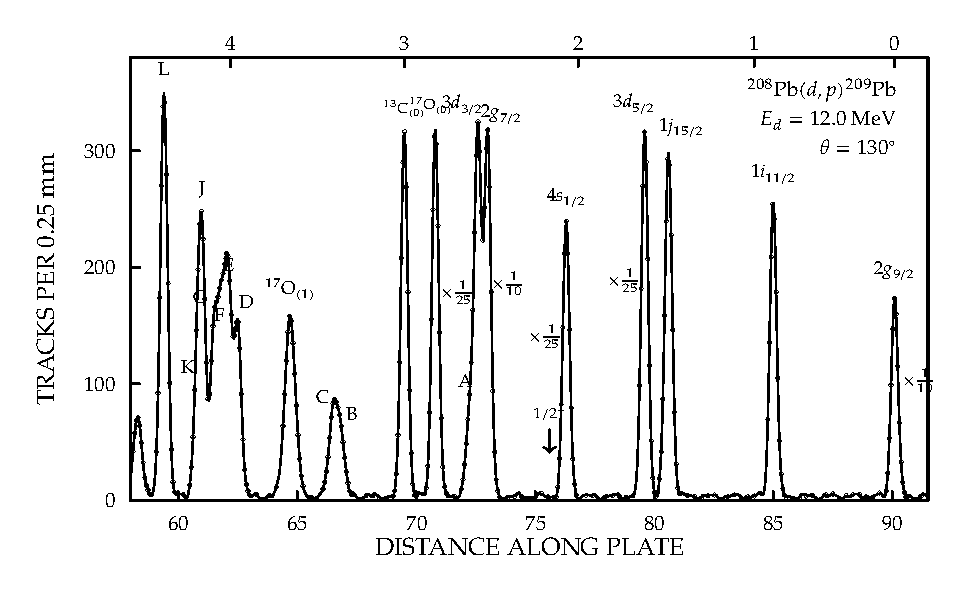
\includegraphics[width=0.75\textwidth]{pictures/2_14}
\par\end{centering}
\caption{\label{fig:2_14}图 2.14 来自 \$\textasciicircum\{208\}}
\end{figure}

\begin{itemize}
\item 准自由散射敲出反应：高能 $(p,2p)$ 与 $(e,e'p)$ 反应能够直接测量原子核深层束缚轨道的单粒子能谱和动量分布（图
2.11 与图 2.13）。
\end{itemize}
\begin{figure}[H]
\begin{centering}
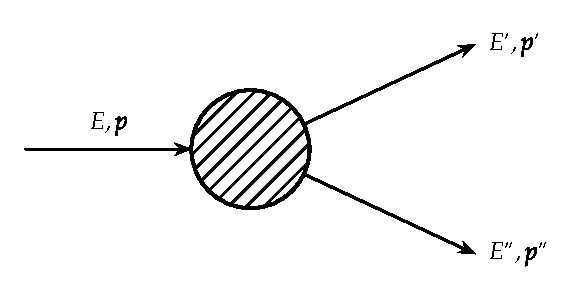
\includegraphics[width=0.75\textwidth]{pictures/2_11}
\par\end{centering}
\caption{\label{fig:2_11}图 2.11 准自由敲出反应 \$(p,2p)\$ 的示意图。}
\end{figure}

在壳模型图像下，被打出核子的束缚能由能量守恒给出：$E_{B}=E-E'-E''$（图 2.12）。

\begin{figure}[H]
\begin{centering}
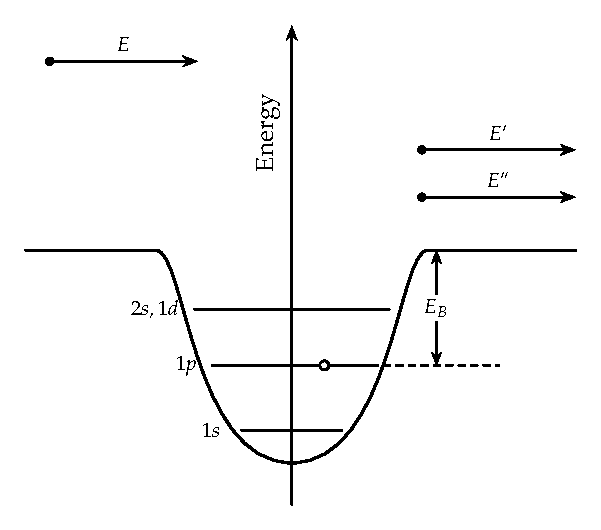
\includegraphics[width=0.75\textwidth]{pictures/2_12}
\par\end{centering}
\caption{\label{fig:2_12}图 2.12 壳模型框架下的 \$(p,2p)\$ 反应过程示意图。}
\end{figure}

\begin{figure}[H]
\begin{centering}
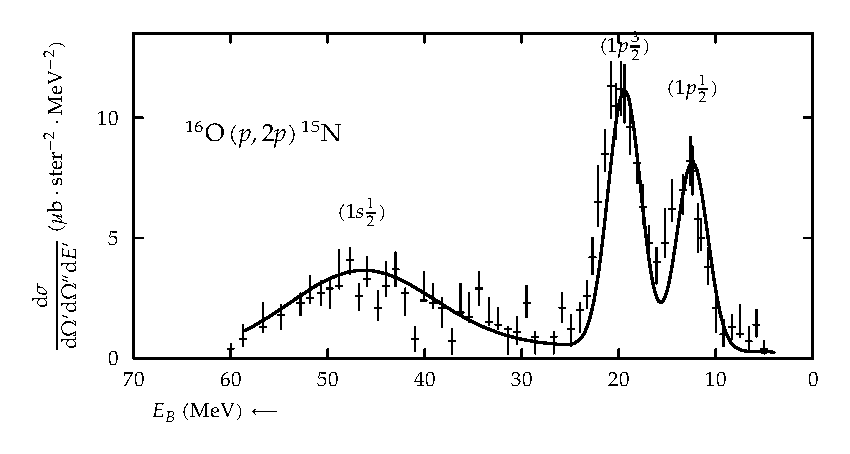
\includegraphics[width=0.75\textwidth]{pictures/2_13}
\par\end{centering}
\caption{\label{fig:2_13}图 2.13 实验测量的 \$\textasciicircum\{16\}}
\end{figure}

图 2.15 给出了双幻核 $\ce{^{208}Pb}$ 邻近奇核（$\ce{^{209}Pb},\ce{^{207}Pb},\ce{^{209}Bi},\ce{^{207}Tl}$）测得的单粒子与单空穴能级同理论
Woods-Saxon 势计算值的对比。实验结果不仅证实了高 $j$ 侵入轨道的存在，而且光谱学因子 $S_{j}\approx1$，说明双闭壳核附近的低激发态确实具有极其纯粹的单粒子特征。远离闭壳时，单粒子强度发生明显的碎裂（Fragmentation），表明单粒子自由度与集体振动（声子）之间存在强烈的粒子-振动耦合（Particle-vibration
coupling）。

\begin{figure}[H]
\begin{centering}
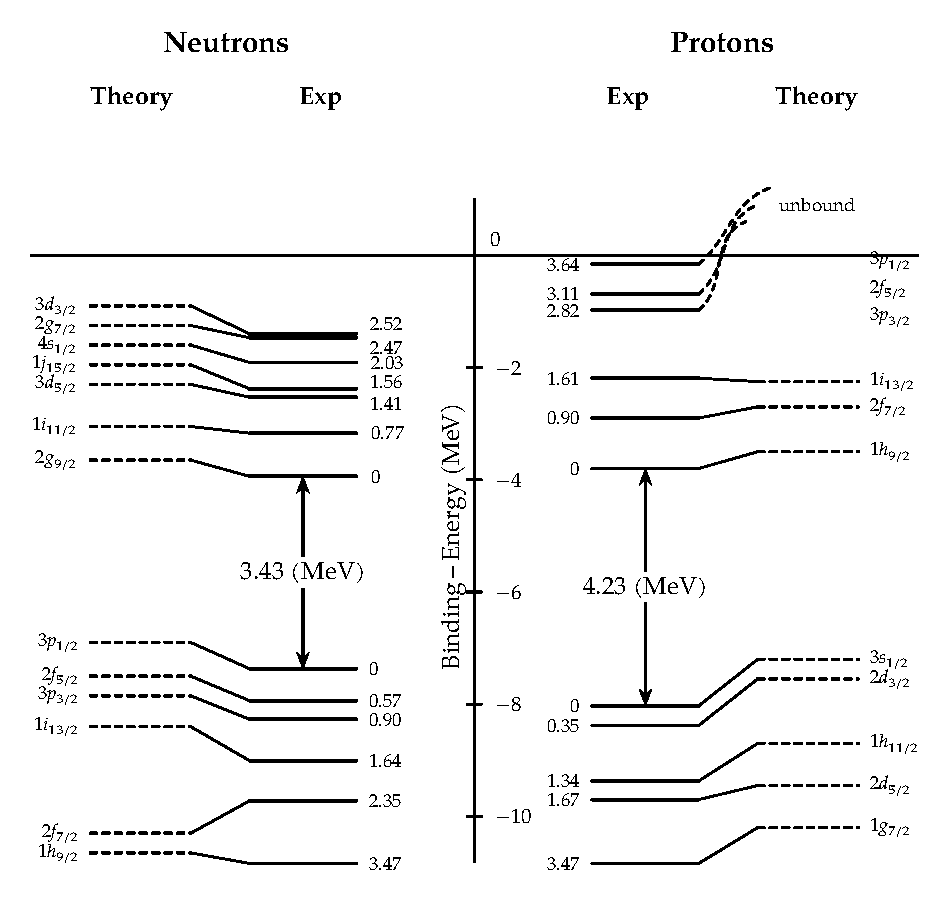
\includegraphics[width=0.75\textwidth]{pictures/2_15}
\par\end{centering}
\caption{\label{fig:2_15}图 2.15 \$\textasciicircum\{208\}}
\end{figure}


\subsection{电磁极矩与跃迁}

单核子电磁极矩与跃迁几率提供了检验核波函数细节的极其敏感的工具（详见附录 B）。

磁偶极矩算符由轨道磁矩与内秉自旋磁矩组成：

\begin{equation}
\boldsymbol{\mu}=\sum^{A}_{i=1}\left(g_{li}\boldsymbol{l}_{i}+g_{si}\boldsymbol{s}_{i}\right)\mu_{N}\label{eq:mag_moment_operator}
\end{equation}

对于单个闭壳外奇核子，在角动量为 $j$ 的状态下计算得到的磁矩被称为 Schmidt 极限（Schmidt limits / Schmidt
lines）\cite{Sc37}：

\begin{align}
\mu & =\left[g_{l}\left(j-\frac{1}{2}\right)+\frac{1}{2}g_{s}\right]\mu_{N},\quad\text{对于 }j=l+\frac{1}{2}\nonumber \\
\mu & =\frac{j}{j+1}\left[g_{l}\left(j+\frac{3}{2}\right)-\frac{1}{2}g_{s}\right]\mu_{N},\quad\text{对于 }j=l-\frac{1}{2}\label{eq:schmidt_limits}
\end{align}

实验测量的磁矩普遍分布在两条 Schmidt 线之间（图 2.17），系统性地小于单粒子预言值（淬灭效应，Quenching）。这一偏差主要源于残余相互作用引起的核芯极化（Core
polarization，即价核子激发闭壳核芯形成粒子-空穴对）以及核子间介子交换流（Meson exchange currents）的贡献。

\begin{figure}[H]
\begin{centering}
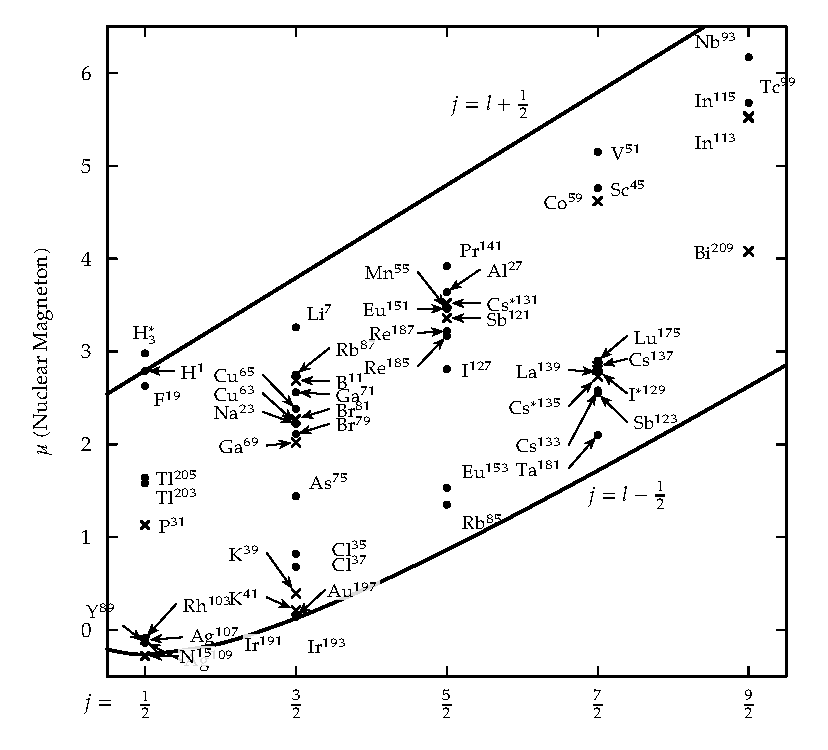
\includegraphics[width=0.75\textwidth]{pictures/2_16}
\par\end{centering}
\caption{\label{fig:2_16}图 2.16 奇 \$Z\$ 核磁矩作为角动量的函数（Schmidt 线，引自 {[}MJ 55{]}）。}
\end{figure}

\begin{figure}[H]
\begin{centering}
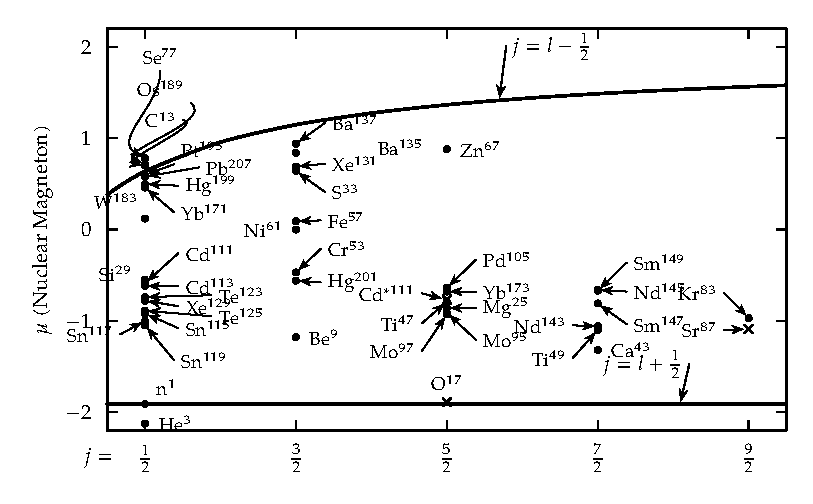
\includegraphics[width=0.75\textwidth]{pictures/2_17}
\par\end{centering}
\caption{\label{fig:2_17}图 2.17 奇 \$N\$ 核磁矩作为角动量的函数（Schmidt 线，引自 {[}MJ 55{]}）。}
\end{figure}

单粒子电四极矩定义为：

\begin{equation}
Q_{\text{s.p.}}=-e_{i}\frac{2j-1}{2(j+1)}\langle r^{2}\rangle\label{eq:single_particle_quadrupole}
\end{equation}

按单纯壳模型，中子不带电（$e_{n}=0$），其实验四极矩应严格为零；而奇质子核的四极矩应由其价质子产生。然而实验测量发现：
\begin{itemize}
\item 奇中子核呈现出明显的非零电四极矩；
\item 奇质子核的实验四极矩比单粒子理论值大近两倍。
\end{itemize}
这一显著效应可以通过引入有效电荷（Effective charge）$e_{\text{eff}}$ 来解释：

\begin{equation}
e_{\text{eff}}=e_{i}+\delta e\label{eq:effective_charge_def}
\end{equation}

其中极化电荷 $\delta e$ 反映了价核子通过两体相互作用将带电核芯极化、激发出虚四极巨共振集体模的效应。在近闭壳核中，典型的极化电荷实验值为：

\begin{equation}
\delta e_{p}\simeq0.5e,\quad\delta e_{n}\simeq0.5e\label{eq:polarization_charge_values}
\end{equation}

由此中子的有效电荷为 $e_{\text{eff}}(n)\simeq0.5e$，质子的有效电荷为 $e_{\text{eff}}(p)\simeq1.5e$。利用这些有效电荷，能够极好地统一解释近闭壳核的静电四极矩以及单粒子电多极跃迁率（以
Weisskopf 单粒子单位 W.u. 衡量）。此外，由于自旋和宇称选择定则的限制，某些高自旋单粒子态只能通过极高多极度的电磁辐射退激发，因而具有极长的寿命，在核素图中形成了著名的“同质异能岛”（Islands
of isomers）。

而在远离闭壳的稀土区和锕系区，实验测量的电四极矩比单粒子预言值大一至两个数量级，且普遍为正值（长椭球形变），清楚表明核芯本身发生了显著的整体稳定形变（图
2.18）。

\begin{figure}[H]
\begin{centering}
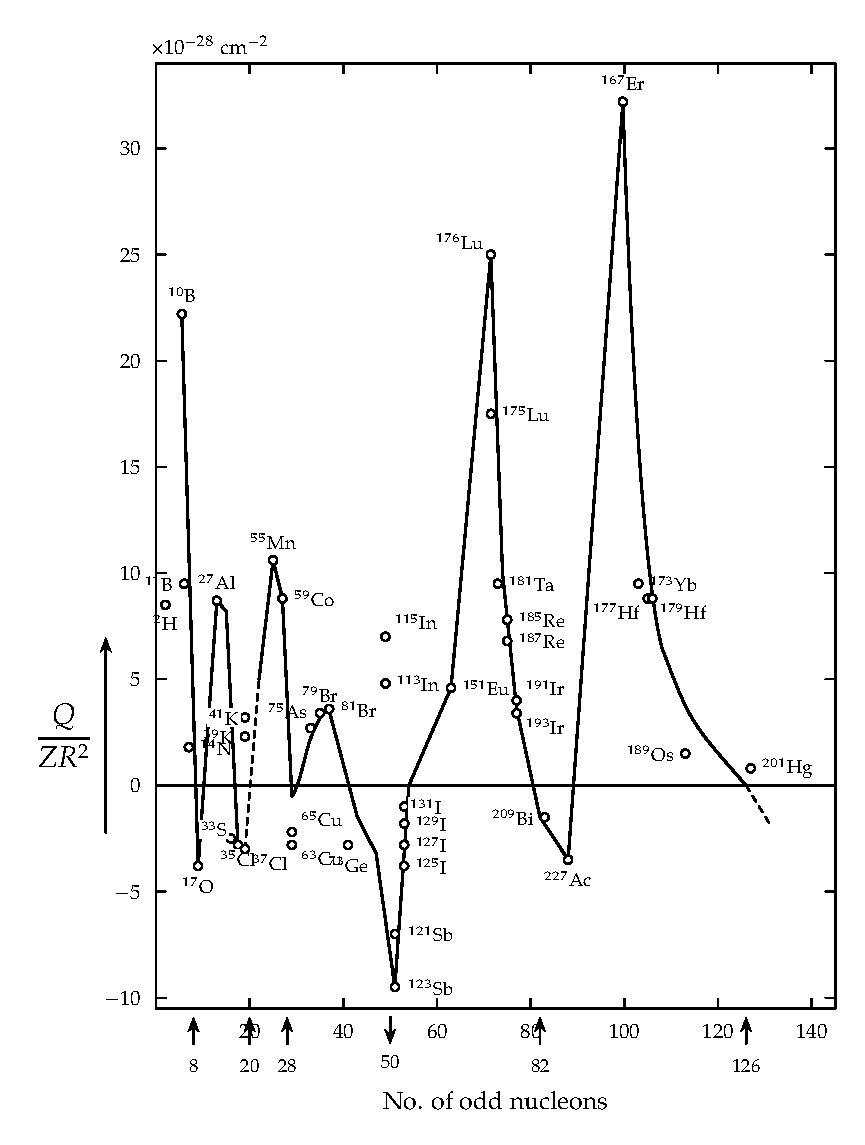
\includegraphics[width=0.75\textwidth]{pictures/2_18}
\par\end{centering}
\caption{\label{fig:2_18}图 2.18 奇 \$A\$ 核电四极矩随奇核子数的变化曲线。箭头标出了满壳位置（引自 {[}Se
64{]}）。}
\end{figure}


\section{形变壳模型\label{sec:=005F62=0053D8=0058F3=006A21=00578B}}

\subsection{实验证据}

在平均势中核子近似独立的运动是壳模型及所有有限核微观理论的基石。在最简单的形式下，该平均势阱被假定为球对称的。这对于闭壳或近闭壳核是高度精确的；然而，当远离闭壳核时，实验观测到了强烈的偏离：
\begin{itemize}
\item 巨大的电四极矩：在稀土区（$150<A<190$）与锕系区（$A>220$），测量到的核基态内秉电四极矩 $Q_{0}$ 比单个未配对核子预期的单粒子值大一到两个数量级（可达数个靶恩，$10^{-24}\,\text{cm}^{2}$）。这意味着有数十个核子协同参与了非球形的形变。
\item 典型的转动能谱：这些核的激发谱呈现出极为规则的转动带序列，其激发能量严格遵循 $E_{I}=\frac{\hbar^{2}}{2\mathcal{J}}I(I+1)$
规律（偶偶核为 $0^{+},2^{+},4^{+},6^{+},\dots$），伴随着极强增强的集体 $E2$ 跃迁（见第 1、3
章）。
\end{itemize}
这些无可辩驳的实验事实清楚地表明，对于开壳层核，原子核的基态自身发生了空间转动对称性的自发破缺，平均场势阱不再保持球形，而形成了固定的空间取向形变。

\subsection{一般的形变势}

描述非球形核表面的普遍方法是将核半径按球谐函数展开：

\begin{equation}
R(\theta,\phi)=R_{0}\left[1+\sum^{\infty}_{\lambda=0}\sum^{\lambda}_{\mu=-\lambda}\alpha^{*}_{\lambda\mu}Y_{\lambda\mu}(\theta,\phi)\right]\label{eq:deformed_surface_expansion}
\end{equation}

其中 $\lambda=1$ 对应质心平移（不改变内秉形状），最重要的多极形变为四极形变 $\lambda=2$。在内秉体固坐标系下，五重分量可由
Hill-Wheeler 形状坐标 $\beta,\gamma$ 参数化（见 1.2 节）：

\begin{align}
a_{20} & =\beta\cos\gamma\nonumber \\
a_{22}=a_{2,-2} & =\frac{1}{\sqrt{2}}\beta\sin\gamma\label{eq:hill_wheeler_beta_gamma}
\end{align}

对于轴对称椭球（$\gamma=0^{\circ}$ 对应长椭球，$\gamma=60^{\circ}$ 对应扁椭球），形变 Woods-Saxon
势具有形式：

\begin{equation}
V(r,\theta,\phi)=-V_{0}\left[1+\exp\left(\frac{r-R(\theta,\phi)}{a(\theta,\phi)}\right)\right]^{-1}\label{eq:deformed_WS_pot}
\end{equation}


\subsection{各向异性谐振子}

若假定形变核的密度为椭球分布，则在谐振子近似下最方便的平均势是各向异性谐振子 Hamilton 量：

\begin{equation}
h_{0}=-\frac{\hbar^{2}}{2m}\nabla^{2}+\frac{m}{2}\left(\omega^{2}_{x}x^{2}+\omega^{2}_{y}y^{2}+\omega^{2}_{z}z^{2}\right)\label{eq:aniso_ho_h0}
\end{equation}

由椭球等势面要求，振荡频率反比于半轴长：$\omega_{\nu}=\omega_{0}\frac{R_{0}}{a_{\nu}}$（$\nu=x,y,z$）。不可压缩流体的体积守恒条件要求：

\begin{equation}
\omega_{x}\omega_{y}\omega_{z}=\text{常数}=\omega^{3}_{0}\label{eq:aniso_ho_vol_conserv}
\end{equation}

本征值为三方向谐振子能量之和：

\begin{equation}
\varepsilon_{0}(n_{x},n_{y},n_{z})=\hbar\omega_{x}\left(n_{x}+\frac{1}{2}\right)+\hbar\omega_{y}\left(n_{y}+\frac{1}{2}\right)+\hbar\omega_{z}\left(n_{z}+\frac{1}{2}\right)\label{eq:aniso_ho_eigenval}
\end{equation}

在轴对称情形下，取 $z$ 轴为对称轴，引入无量纲形变参数 $\delta$：

\begin{align}
\omega^{2}_{\perp}=\omega^{2}_{x}=\omega^{2}_{y} & =\omega^{2}_{0}(\delta)\left(1+\frac{2}{3}\delta\right)\nonumber \\
\omega^{2}_{z} & =\omega^{2}_{0}(\delta)\left(1-\frac{4}{3}\delta\right)\label{eq:aniso_ho_omega_delta}
\end{align}

由体积守恒条件 \ref{eq:aniso_ho_vol_conserv}，展开到 $\delta$ 的二阶可得：

\begin{equation}
\omega_{0}(\delta)=\omega_{0}\left(1+\frac{2}{9}\delta^{2}\right)\label{eq:omega_delta_order2}
\end{equation}

引入形变依赖的特征振子长度 $b(\delta)=\sqrt{\hbar/(m\omega_{0}(\delta))}$ 及无量纲坐标
$\boldsymbol{r}'=\boldsymbol{r}/b(\delta)$，Hamilton 量可表示为球形谐振子加上四极形变扰动项：

\begin{equation}
h_{0}(\delta)=\hbar\omega_{0}(\delta)\left(-\frac{1}{2}\nabla'^{2}+\frac{1}{2}r'^{2}-\frac{1}{3}\sqrt{\frac{16\pi}{5}}\,\delta\,r'^{2}Y_{20}(\theta',\phi')\right)\label{eq:dimensionless_aniso_ho}
\end{equation}

\begin{figure}[H]
\begin{centering}
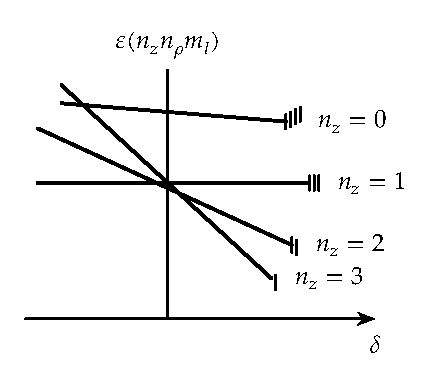
\includegraphics[width=0.75\textwidth]{pictures/2_19}
\par\end{centering}
\caption{\label{fig:2_19}图 2.19 各向异性谐振子能级作为形变参数 \$}
\end{figure}


\subsection{Nilsson Hamilton量}

单纯的形变谐振子势无法给出正确的自旋-轨道劈裂以及重核内部平坦底部的势阱特征。为了在形变核中再现真实的单粒子能谱，Nilsson \cite{Ni55}
在形变谐振子基底上引入了自旋-轨道耦合项与角动量修正项：

\begin{equation}
h=h_{0}(\delta)-\kappa\hbar\omega_{0}\left[2\boldsymbol{l}\cdot\boldsymbol{s}+\mu\left(\boldsymbol{l}^{2}-\langle\boldsymbol{l}^{2}\rangle_{N}\right)\right]\label{eq:nilsson_hamiltonian}
\end{equation}

其中 $\kappa$ 决定了自旋-轨道相互作用的强度，$\mu$ 调节高 $l$ 轨道的相对能量（模拟势阱底部的平坦化），常数
$\langle\boldsymbol{l}^{2}\rangle_{N}=\frac{1}{2}N(N+3)$ 保证各主振子壳层能量重心不发生整体漂移。

\begin{figure}[H]
\begin{centering}
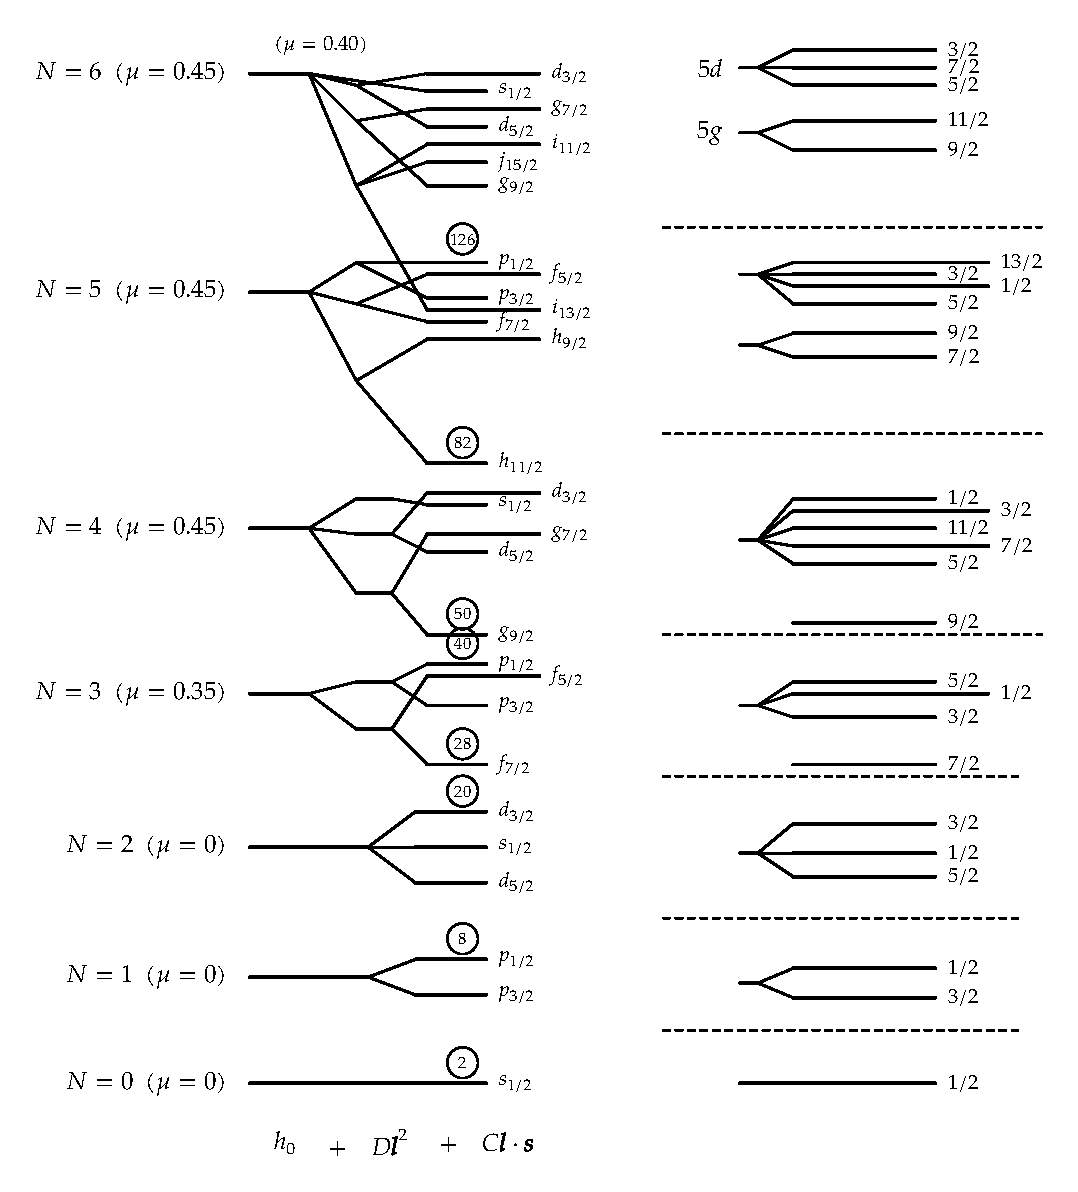
\includegraphics[width=0.75\textwidth]{pictures/2_20}
\par\end{centering}
\caption{\label{fig:2_20}图 2.20 借助 \$}
\end{figure}

由于形变势破坏了全空间转动球对称性，总角动量 $j$ 不再是好量子数。但对于轴对称核，绕对称轴（$z$ 轴）的转动不变性与空间宇称仍然保持守恒。因此总角动量在
$z$ 轴上的投影 $\Omega$ 与空间宇称 $\pi=(-1)^{N}$ 是严格的好量子数：

\begin{equation}
\Omega=j_{z}=l_{z}+s_{z}=\Lambda+\Sigma\label{eq:nilsson_omega_def}
\end{equation}

在大形变极限下，单粒子能级可以用柱坐标下的渐近基量子数 $|Nn_{z}\Lambda\Omega\rangle$（通常简写为渐近标记
$[Nn_{z}\Lambda\Omega]$）标记，其中：
\begin{itemize}
\item $N$：主谐振子量子数；
\item $n_{z}$：沿对称轴方向的振动激发量子数（$n_{z}$ 越大，轨道波函数沿 $z$ 轴越延展，长椭球形变时能量随 $\delta$
下降越快）；
\item $\Lambda$：轨道角动量在 $z$ 轴上的投影（$\Lambda=N-n_{z},N-n_{z}-2,\dots$）；
\item $\Omega=\Lambda\pm1/2$：总角动量在 $z$ 轴上的投影。
\end{itemize}
根据量子力学的不交叉定则（No-crossing rule），具有相同对称性量子数（相同 $\Omega$ 与相同宇称 $\pi$）的能级随形变变化时不会真正相交，而是发生强烈的组态混杂并彼此排斥；只有具有不同
$\Omega$ 或不同宇称的能级才能自由相交。图 2.21 展示了著名的 Nilsson 能级图。

\begin{figure}[H]
\begin{centering}
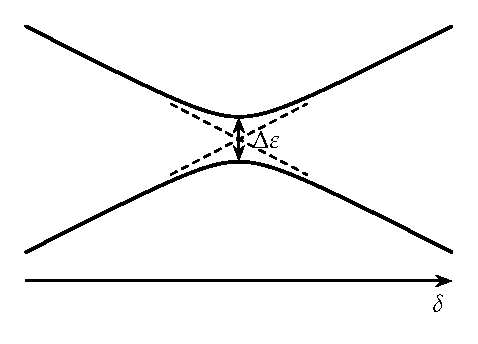
\includegraphics[width=0.75\textwidth]{pictures/2_22}
\par\end{centering}
\caption{\label{fig:2_22}图 2.22 具有相同对称性的两个能级的不相交定则（Neumann-Wigner 定则）。}
\end{figure}

\begin{figure}[H]
\begin{centering}
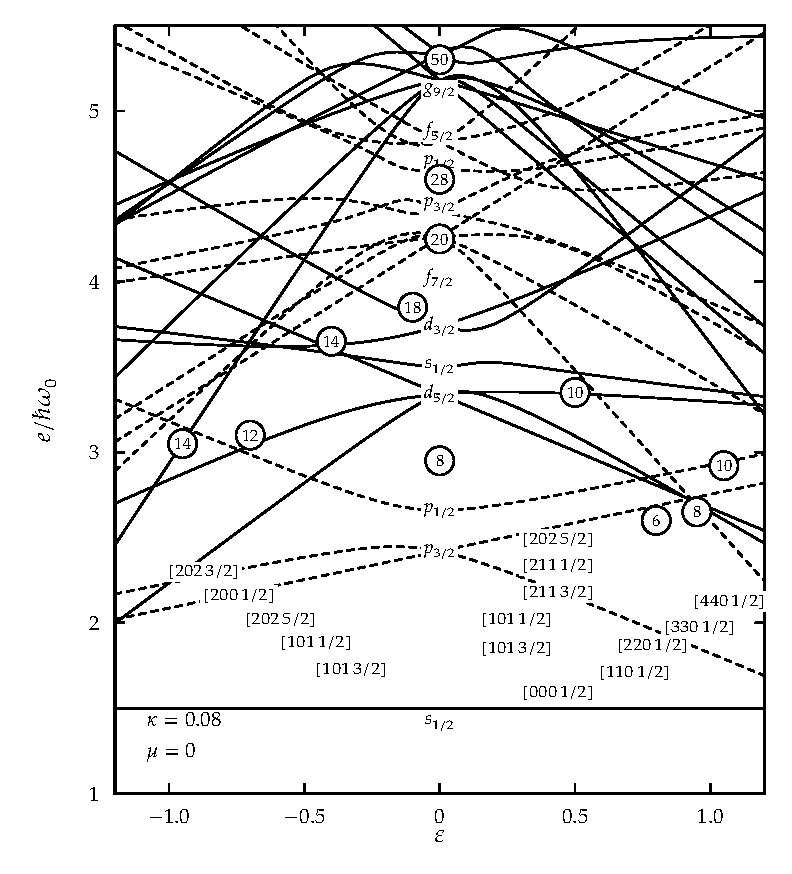
\includegraphics[width=0.75\textwidth]{pictures/2_21a}
\par\end{centering}
\caption{\label{fig:2_21a}图 2.21a 轻核区的 Nilsson 模型单粒子能级图。}
\end{figure}

\begin{figure}[H]
\begin{centering}
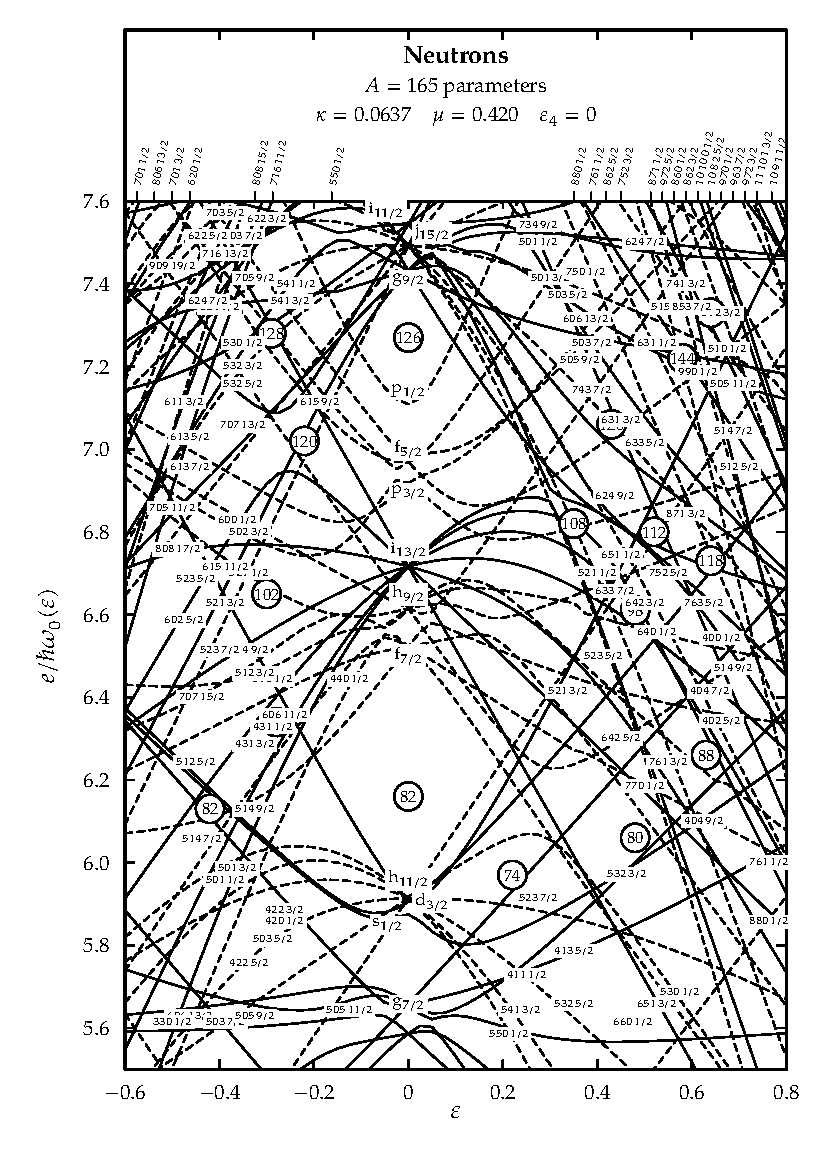
\includegraphics[width=0.75\textwidth]{pictures/2_21b}
\par\end{centering}
\caption{\label{fig:2_21b}图 2.21b 重核区中子的 Nilsson 模型单粒子能级图。}
\end{figure}

\begin{figure}[H]
\begin{centering}
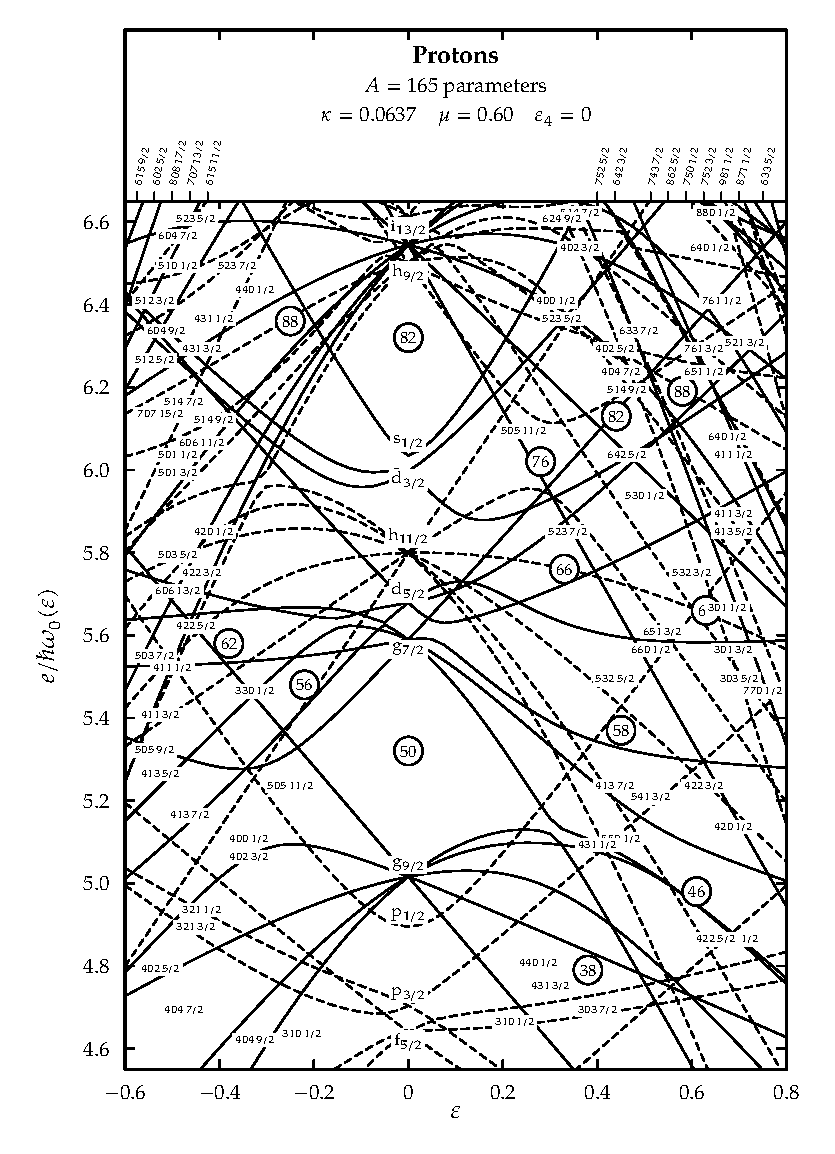
\includegraphics[width=0.75\textwidth]{pictures/2_21c}
\par\end{centering}
\caption{\label{fig:2_21c}图 2.21c 重核区质子的 Nilsson 模型单粒子能级图。}
\end{figure}


\subsection{奇核基态的量子数}

根据时间反演对称性（Kramers 简并），每个形变能级 $\pm\Omega$ 严格二重简并。因此在形变核基态中，所有成对的质子或中子分别以时间反演共轭的方式配对填入
Nilsson 轨道，其总角动量在对称轴上的投影和为零。

对于奇 $A$ 核，最后一个未配对核子占据最高的 Nilsson 能级，因此形变核基态的自旋与宇称完全由该孤立单粒子的 Nilsson
态决定：

\begin{equation}
I=\Omega,\quad\pi=(-1)^{N}\label{eq:nilsson_odd_ground_spin}
\end{equation}

这一简单的定则在稀土区和锕系区的数百个形变奇核中获得了令人惊叹的成功，绝大多数实验测得的基态自旋和宇称均与 Nilsson 能级序列的理论预言完全一致。

\begin{figure}[H]
\begin{centering}
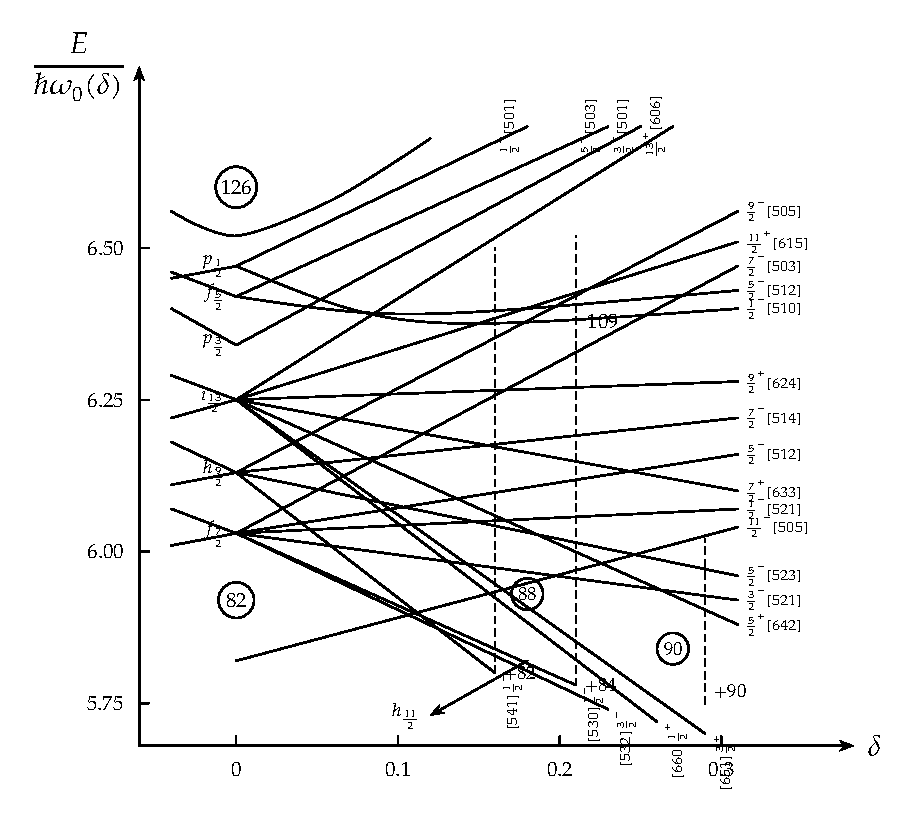
\includegraphics[width=0.75\textwidth]{pictures/2_23}
\par\end{centering}
\caption{\label{fig:2_23}图 2.23 确定奇 \$A\$ 核 \$\textasciicircum\{183\}}
\end{figure}


\subsection{形变能的计算与双中心壳模型}

利用 Nilsson 势最直接的尝试是计算单粒子能量之和随形变参数 $\delta$ 的依赖关系：

\begin{equation}
E_{\text{s.p.}}(\delta)=\sum^{A}_{i=1}\varepsilon_{i}(\delta)\label{eq:sum_single_particle_energy}
\end{equation}

由此寻找能量极小点 $\delta_{\text{eq}}$。虽然这一简单方法对于预测稀土区核的基态平衡形变获得了定性甚至半定量的合理结果（图
2.24），但若将其用于全核素区或大形变行为，就会暴露严重的内在缺陷：

\begin{figure}[H]
\begin{centering}
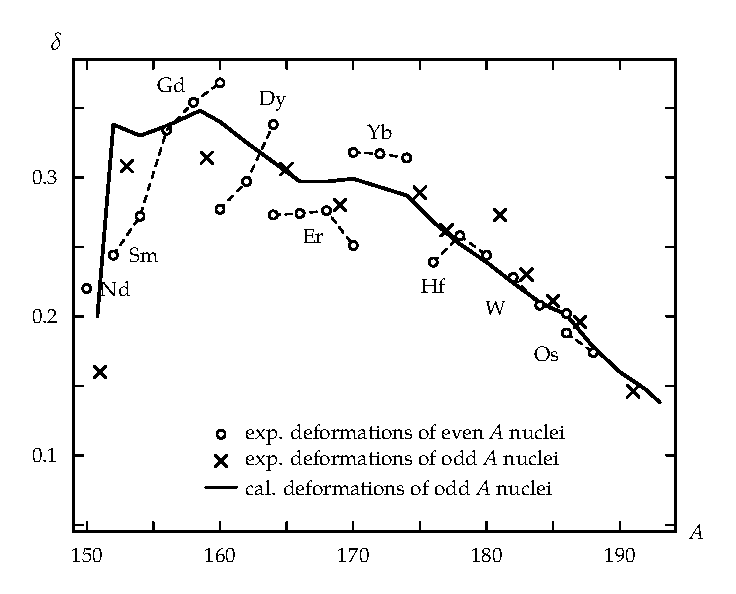
\includegraphics[width=0.75\textwidth]{pictures/2_24}
\par\end{centering}
\caption{\label{fig:2_24}图 2.24 理论计算与实验测定的平衡形变参数比较（引自 {[}MN 55{]}）。}
\end{figure}

\begin{itemize}
\item 能量过度束缚且绝对结合能完全失真：单粒子能量之和 $\sum\varepsilon_{i}$ 重复计算了双体相互作用能（见第 5
章式 (5.28)），导致平均势的体积饱和行为失真；
\item 在大形变与核裂变区域发散：当原子核拉长至发生颈缩、甚至断裂为两个分离的核碎片时，基于单一中心展开的 Nilsson 势完全失去了物理意义。
\end{itemize}
为了描述大形变动力学、重离子聚变与核裂变（Fission）过程，必须构建具有正确渐近极限的形变势模型，其中最重要的代表是双中心壳模型（Two-Center
Shell Model, TCSM）\cite{DR66,HMG69,ADD70,GMG71,MG72}：

双中心模型将平均谐振子势推广为包含两个空间分离中心（位于 $z=\pm z_{0}$）的势阱：

\begin{equation}
V_{\text{TCSM}}(\boldsymbol{r})=\frac{1}{2}m\omega^{2}_{z}(|z|-z_{0})^{2}+\frac{1}{2}m\omega^{2}_{\perp}(x^{2}+y^{2})\label{eq:tcsm_potential}
\end{equation}

当双中心间距 $z_{0}\to0$ 时，势阱平滑过渡为单体复合核的各向异性谐振子势；当 $z_{0}\to\infty$ 时，势阱渐近分解为两个完全独立的单核碎片势。通过在此类具有颈缩参数的双中心势中加入自旋-轨道耦合与形变修正，能够严谨地计算裂变通道上的微观单粒子轨道演化（图
2.25）。类似的大形变势阱还包括折积 Yukawa 势（Folded Yukawa Potential \cite{BFN72,MN73}）和广义形变
Woods-Saxon 势 \cite{BDJ72,Pa73}。

然而，要从这些微观单粒子能级中准确提取真实的形变势能曲面和裂变势垒，必须摒弃粗糙的单粒子能简单求和，而采用宏观-微观结合的 Strutinsky
壳修正方法，这正是下一节的核心主题。

此外在大形变下，微观单粒子壳修正与宏观液滴势垒的叠加，导致能量随形变出现第二极小，完美解释了裂变同质异能现象（图 2.26）。

\begin{figure}[H]
\begin{centering}
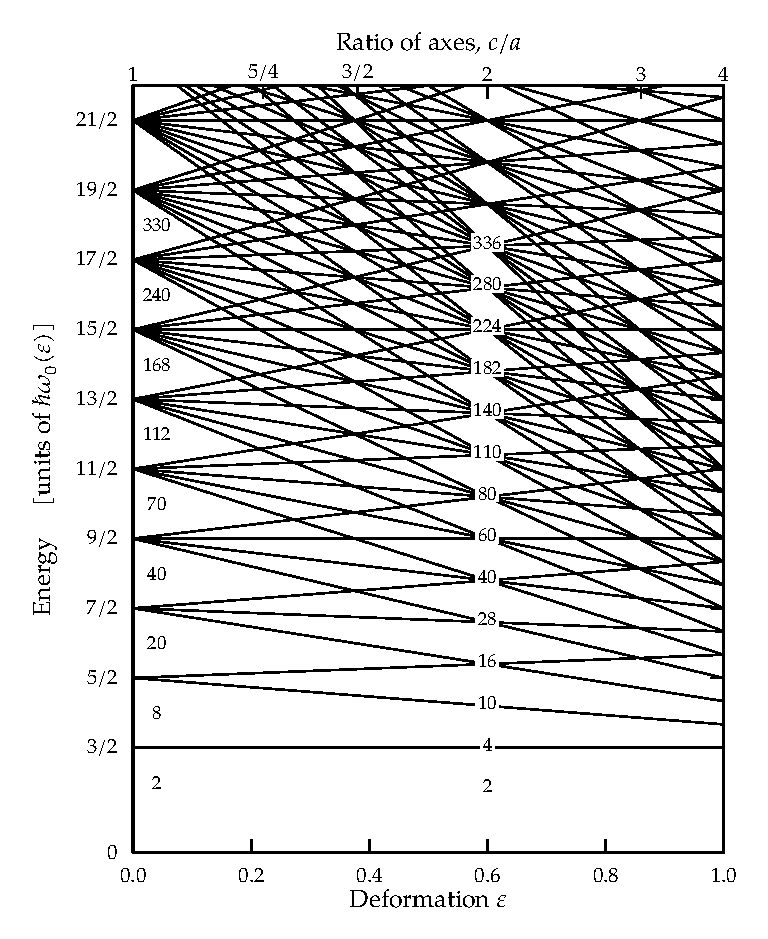
\includegraphics[width=0.75\textwidth]{pictures/2_25}
\par\end{centering}
\caption{\label{fig:2_25}图 2.25 长椭球形变谐振子势中的单粒子能级随形变 \$}
\end{figure}

\begin{figure}[H]
\begin{centering}
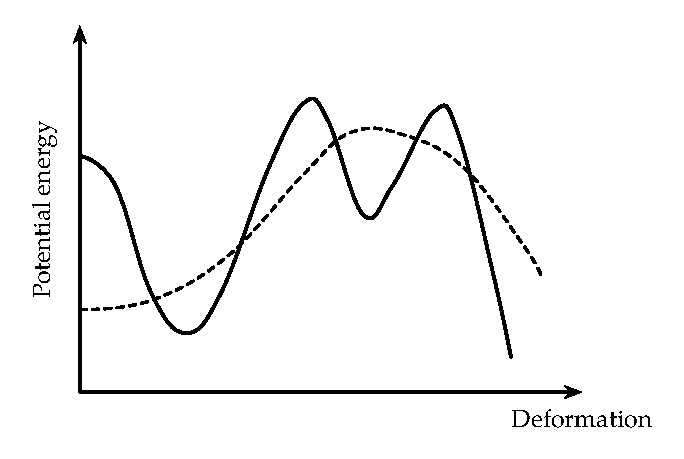
\includegraphics[width=0.75\textwidth]{pictures/2_26}
\par\end{centering}
\caption{\label{fig:2_26}图 2.26 具有第二极小的原子核能量随形变变化的示意图。虚线对应纯液滴模型势垒。}
\end{figure}


\section{液滴模型的壳修正与 Strutinsky 方法\label{sec:=006DB2=006EF4=006A21=00578B=007684=0058F3=004FEE=006B63}}

\subsection{引言}

在第 1 章中我们看到，液滴模型能够极好地再现结合能的平均行为。然而，在幻数附近结合能存在明显的偏离（见图 2.2），这一事实清楚地表明了单粒子壳效应的存在。另一方面，虽然唯象壳模型能够成功解释基态自旋、宇称以及低激发谱的单粒子性质，但如果仅仅将独立单粒子能级之和作为核的总结合能，在定量上却无法给出正确的核物质饱和性质与绝对结合能（如
2.8.6 节所述）。

为了克服这一困难，Strutinsky \cite{St67,St68} 提出了一个非常富有成果的微观-宏观结合方法（宏观-微观方法）。其基本物理图像是：总结合能可以分解为一个平滑变化的大体部分（即宏观液滴模型能量）加上一个由单粒子能级非均匀分布引起的微小涨落修正部分（即微观壳修正能）：

\[
E=E_{\text{LDM}}+E_{\text{osc}}
\]

这种分解基于如下事实：结合能的平均行为主要由平滑的平均能级密度决定，而液滴模型已经通过唯象参数的拟合极好地包含了这部分宏观体积和表面能量；唯象壳模型中不准确的正是其平滑宏观部分，但它却相当精确地给出了
Fermi 能量附近的能级成团结构（即壳效应）。因此，我们只需利用壳模型计算振荡修正量 $E_{\text{osc}}$，并将其加到宏观的液滴模型能量
$E_{\text{LDM}}$ 之上。

\subsection{Strutinsky 平均方法的基本思想}

\begin{figure}[H]
\begin{centering}
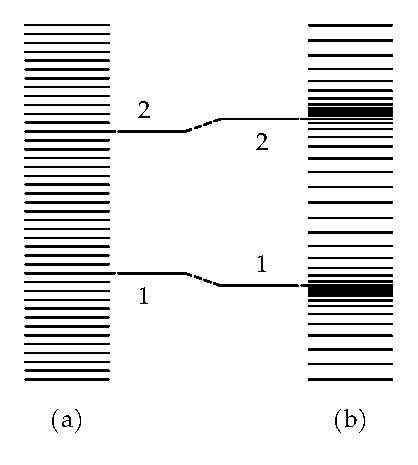
\includegraphics[width=0.75\textwidth]{pictures/2_27}
\par\end{centering}
\caption{\label{fig:2_27}图 2.27 等间距能级密度与示意壳模型聚束能级密度的比较。}
\end{figure}

为了在数学上严谨地定义振荡能量 $E_{\text{osc}}$，首先需要将壳模型的单粒子能级密度 $g(\varepsilon)=\sum_{i}\delta(\varepsilon-\varepsilon_{i})$
分解为平滑部分 $\tilde{g}(\varepsilon)$ 与振荡涨落部分 $\delta g(\varepsilon)$：

\begin{equation}
g(\varepsilon)=\tilde{g}(\varepsilon)+\delta g(\varepsilon)\label{eq:strut_g_decomp}
\end{equation}

由平滑能级密度 $\tilde{g}(\varepsilon)$，可以通过核子数守恒条件唯一定义平滑的化学势（即平均 Fermi
能）$\tilde{\lambda}$：

\begin{equation}
A=\int^{\tilde{\lambda}}_{-\infty}\tilde{g}(\varepsilon)\,\mathrm{d}\varepsilon\label{eq:strut_lambda_tilde}
\end{equation}

由此可得壳模型的平滑能量贡献：

\begin{equation}
\tilde{E}_{\text{sh}}=\int^{\tilde{\lambda}}_{-\infty}\varepsilon\,\tilde{g}(\varepsilon)\,\mathrm{d}\varepsilon\label{eq:strut_E_smooth}
\end{equation}

而单纯单粒子壳模型给出的基态能量为：

\begin{equation}
E_{\text{sh}}=\sum^{A}_{i=1}\varepsilon_{i}\label{eq:strut_E_sh}
\end{equation}

因此，由于壳层非均匀聚集导致的能量涨落（壳修正能）即为二者之差：

\begin{equation}
E_{\text{osc}}=E_{\text{sh}}-\tilde{E}_{\text{sh}}\label{eq:strut_E_osc_def}
\end{equation}

由此体系的总能量表示为：

\begin{equation}
E=E_{\text{LDM}}+E_{\text{sh}}-\tilde{E}_{\text{sh}}\label{eq:strut_total_E}
\end{equation}

在液滴模型中，稳定的平衡核形状总是球对称的。但由于额外的壳修正项 $E_{\text{osc}}$ 随形变剧烈振荡，在核素表的许多区域（如稀土区与锕系区），Strutinsky
平均能量式 \ref{eq:strut_total_E} 的能量极小值将落在非零的形变处，从而自然地解释了原子核的自发四极形变。

\subsection{平均能级密度的确定}

现在我们探讨如何从给定的离散单粒子能级谱 $g(\varepsilon)=\sum_{i}\delta(\varepsilon-\varepsilon_{i})$
中，以严格的数学方式提取其平滑部分 $\tilde{g}(\varepsilon)$。困难在于三维势阱中的能级密度随能量呈现非线性增长，且聚集成间距约为
$\hbar\omega_{0}$ 的壳层。通常的想法是将能级密度与一个平滑函数 $f(x)$ 进行折积：

\begin{equation}
\tilde{g}(\varepsilon)=\frac{1}{\gamma}\int^{+\infty}_{-\infty}g(\varepsilon')f\left(\frac{\varepsilon'-\varepsilon}{\gamma}\right)\,\mathrm{d}\varepsilon'\label{eq:strut_folding}
\end{equation}

\begin{figure}[H]
\begin{centering}
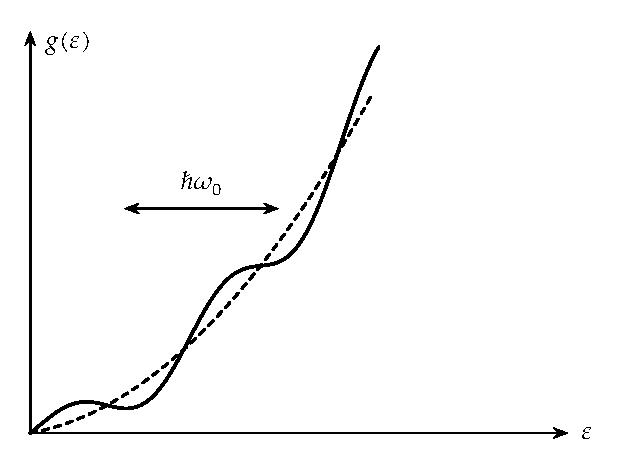
\includegraphics[width=0.75\textwidth]{pictures/2_28}
\par\end{centering}
\caption{\label{fig:2_28}图 2.28 三维无限深势阱中能级密度的示意图（展示离散尖峰能级密度与平滑平均能级密度）。}
\end{figure}

其中 $\gamma$ 为平滑宽度，其大小取为主壳层间隔量级（$\gamma\simeq\hbar\omega_{0}$）。然而单纯取
$f$ 为纯 Gauss 函数并不充分，因为合理的平滑程序必须满足自洽重平均不变性：若对已经平滑的能级密度 $\tilde{g}$
再次施行相同的平滑操作，其结果应保持不变：

\begin{equation}
\tilde{g}(\varepsilon)=\frac{1}{\gamma}\int^{+\infty}_{-\infty}\tilde{g}(\varepsilon')f\left(\frac{\varepsilon'-\varepsilon}{\gamma}\right)\,\mathrm{d}\varepsilon'\label{eq:strut_self_consistent}
\end{equation}

当 $f$ 为纯 Gauss 函数而 $\tilde{g}$ 包含多项式曲率时，式 \ref{eq:strut_self_consistent}
并不严格成立。由于积分的主要贡献来自于 $\varepsilon'=\varepsilon$ 的近邻区域，我们假定平滑密度 $\tilde{g}(\varepsilon')$
在局域上可以被一个 $2M$ 阶的多项式很好地逼近（通常取 $2M=2,4,6$）。此时若将平滑函数取为多项式与加权因子的乘积：

\begin{equation}
f(x)=P(x)w(x)\label{eq:strut_f_pw}
\end{equation}

其中 $P(x)$ 为 $2M$ 阶偶多项式（曲率修正多项式），$w(x)$ 为 Gauss 加权函数：

\begin{equation}
w(x)=\frac{1}{\sqrt{\pi}}e^{-x^{2}}\label{eq:strut_gauss_w}
\end{equation}

通过正交多项式理论 \cite{AS65}，$P(x)$ 可以由 Hermite 多项式精确构建：

\begin{equation}
P(x)=\sum^{M}_{n=0}\frac{(-1)^{n}}{2^{2n}n!}H_{2n}(x)=L^{1/2}_{M}(x^{2})\label{eq:strut_laguerre}
\end{equation}

这里 $L^{1/2}_{M}(x^{2})$ 是伴随 Laguerre 多项式。展开为幂级数形式：

\begin{equation}
L^{1/2}_{M}(x^{2})=\sum^{M}_{n=0}a_{2n}x^{2n}\label{eq:strut_laguerre_poly}
\end{equation}

在实际计算中常用的前四阶系数如表 2.5 所示。

\begin{table}[htbp]
\caption{\label{tab:laguerre_coefficients}前四个 Laguerre 多项式系数}

\centering{}%
\begin{tabular}{ccccc}
\hline 
$M$ & $a_{0}$ & $a_{2}$ & $a_{4}$ & $a_{6}$\tabularnewline
\hline 
0 & 1 & — & — & —\tabularnewline
1 & 3/2 & -1 & — & —\tabularnewline
2 & 15/8 & -5/2 & 1/2 & —\tabularnewline
3 & 35/16 & -35/8 & 7/4 & -1/6\tabularnewline
\hline 
\end{tabular}
\end{table}

接下来需要确定平滑参数 $\gamma$ 与曲率阶数 $M$ 的具体取值。物理上有意义的平均方法必须要求最终计算出的物理量在很大程度上独立于平滑参数的选择。这意味着对于固定的
$M$，平均能量 $\tilde{E}_{\text{sh}}$ 随 $\gamma$ 的变化必须存在一个平坦的“坪区”（Plateau），在该区域内严格满足坪区条件
\cite{BP73}：

\begin{equation}
\frac{\partial\tilde{E}_{\text{sh}}}{\partial\gamma}=0\label{eq:strut_plateau}
\end{equation}

由于真实核能级总是以大约 $\hbar\omega_{0}$ 的间距成团，只要取 $\gamma\simeq(1.0\sim1.5)\hbar\omega_{0}$
且 $M\geqslant2$，在绝大多数核物理问题中均能观察到极为宽阔稳定的能量坪区。第 13 章将进一步证明，Strutinsky
平滑方法在深层次上与半经典 Thomas-Fermi 近似完全等价。

\begin{figure}[H]
\begin{centering}
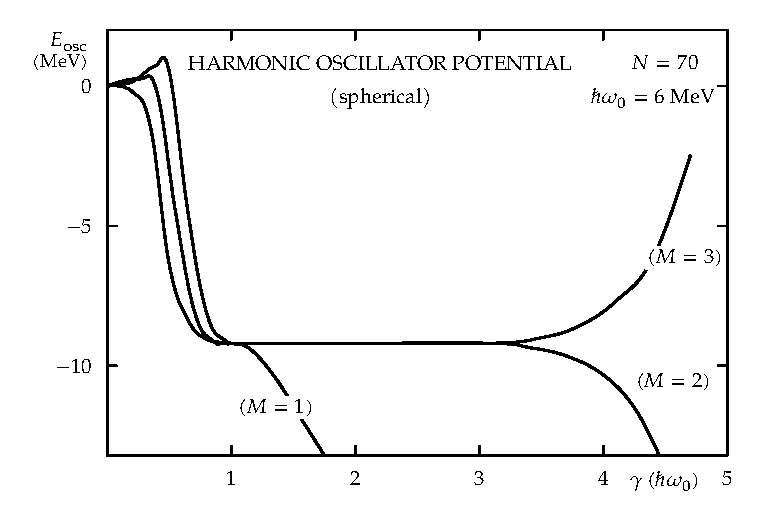
\includegraphics[width=0.75\textwidth]{pictures/2_30}
\par\end{centering}
\caption{\label{fig:2_30}图 2.30 谐振子势的壳修正能作为平滑宽度 \$}
\end{figure}


\subsection{Strutinsky 壳修正能的计算}

利用确定的平滑函数 $f(x)$，由离散谱 $g(\varepsilon)=\sum_{i}\delta(\varepsilon-\varepsilon_{i})$
得到的平滑能级密度为：

\begin{equation}
\tilde{g}(\varepsilon)=\sum_{i}\frac{1}{\gamma}f\left(\frac{\varepsilon-\varepsilon_{i}}{\gamma}\right)\label{eq:strut_g_smooth_sum}
\end{equation}

将其代入粒子数积分，可引入广义占据数 $\tilde{n}_{i}$：

\begin{equation}
A=\sum_{i}\tilde{n}_{i}=\sum_{i}\int^{t_{i}}_{-\infty}f(x)\,\mathrm{d}x,\quad t_{i}=\frac{\tilde{\lambda}-\varepsilon_{i}}{\gamma}\label{eq:strut_n_tilde}
\end{equation}

由此平滑能量可写为：

\begin{equation}
\tilde{E}_{\text{sh}}=\sum_{i}\varepsilon_{i}\tilde{n}_{i}+F\label{eq:strut_E_smooth_F}
\end{equation}

其中残余项 $F$ 为：

\begin{equation}
F=\sum_{i}\int^{\tilde{\lambda}}_{-\infty}(\varepsilon-\varepsilon_{i})\frac{1}{\gamma}f\left(\frac{\varepsilon-\varepsilon_{i}}{\gamma}\right)\,\mathrm{d}\varepsilon=\gamma\sum_{i}\int^{t_{i}}_{-\infty}xf(x)\,\mathrm{d}x\label{eq:strut_F_def}
\end{equation}

对平滑能量对 $\gamma$ 求导可得：

\begin{equation}
\frac{\partial\tilde{E}_{\text{sh}}}{\partial\gamma}=\frac{1}{\gamma}F+\tilde{\lambda}\frac{\partial}{\partial\gamma}\sum_{i}\tilde{n}_{i}=\frac{1}{\gamma}F+\tilde{\lambda}\frac{\partial A}{\partial\gamma}=\frac{1}{\gamma}F\label{eq:strut_dE_dgamma}
\end{equation}

由于核子数 $A$ 严格守恒（$\partial A/\partial\gamma=0$），坪区条件 $\partial\tilde{E}_{\text{sh}}/\partial\gamma=0$
恰好等价于 $F=0$！定义纯壳模型的阶梯占据数：

\begin{equation}
n_{i}=\begin{cases}
1, & \varepsilon_{i}\leqslant\varepsilon_{F}\\
0, & \varepsilon_{i}>\varepsilon_{F}
\end{cases}\label{eq:strut_step_n}
\end{equation}

则总壳修正能 $E_{\text{osc}}$ 可以极为优美简洁地表示为占据数偏差 $\delta n_{i}=n_{i}-\tilde{n}_{i}$
的单粒子能级加权和：

\begin{equation}
E_{\text{osc}}=\sum_{i}\varepsilon_{i}(n_{i}-\tilde{n}_{i})=\sum_{i}\varepsilon_{i}\delta n_{i}\label{eq:strut_E_osc_final}
\end{equation}

\begin{figure}[H]
\begin{centering}
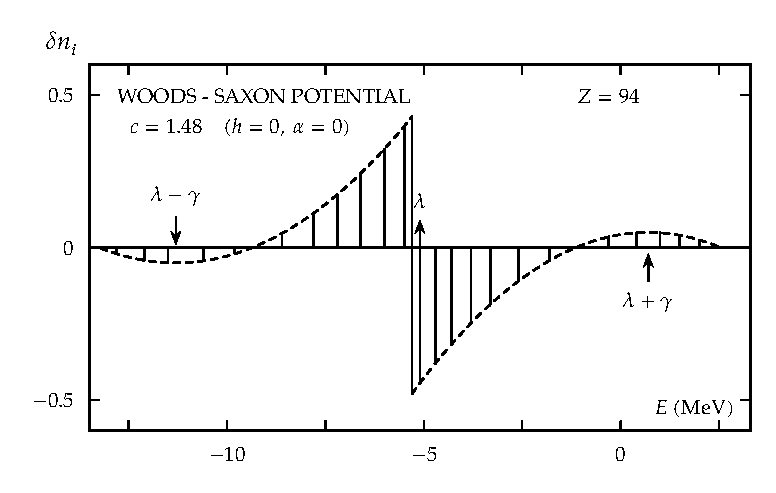
\includegraphics[width=0.75\textwidth]{pictures/2_29}
\par\end{centering}
\caption{\label{fig:2_29}图 2.29 采用 Strutinsky 平均方法对 Woods-Saxon 势计算得到的占有数偏差
\$}
\end{figure}

由占据数偏差量 $\delta n_{i}$，还可以直接计算坐标表象中的微观单体密度壳修正 \cite{Di71}：

\begin{equation}
\delta\rho_{\text{osc}}(\boldsymbol{r},\boldsymbol{r}')=\sum_{i}\phi_{i}(\boldsymbol{r})\phi^{*}_{i}(\boldsymbol{r}')\delta n_{i}\label{eq:strut_delta_rho}
\end{equation}

对于重核，核子对关联（见第 6、7 章）也扮演着重要角色。在 BCS 理论下，对能 $P$ 同样与 Fermi 面附近的能级密度紧密相关。由于宏观液滴能量已拟合了平均质量，其本身已包含了对能的平滑宏观部分
$\tilde{P}_{\text{BCS}}$，因此只需额外加上对能的振荡修正 $P_{\text{osc}}=P_{\text{BCS}}-\tilde{P}_{\text{BCS}}$。最终核体系的总形变能量由下式给出：

\begin{equation}
E=E_{\text{LDM}}+E_{\text{sh}}-\tilde{E}_{\text{sh}}+P_{\text{BCS}}-\tilde{P}_{\text{BCS}}\label{eq:strut_total_E_pairing}
\end{equation}


\subsection{壳修正与 Hartree-Fock 方法}

在第 5 章中我们将详细探讨如何从微观现实核力通过 Hartree-Fock（HF）方法自洽求解微观平均场。在此我们简要说明：Strutinsky
壳修正方法并非唯象拼凑，而是具有坚实的微观理论基础。

在 HF 理论中，基态总能量以表象无关的方式表示为：

\begin{equation}
E^{\text{HF}}_{0}=\mathrm{Tr}(t\rho)+\frac{1}{2}\mathrm{Tr}_{1}\mathrm{Tr}_{1}\rho\bar{v}\rho\label{eq:strut_E_HF}
\end{equation}

其中 $\rho$ 为自洽单粒子密度矩阵，$h^{\text{HF}}=t+\mathrm{Tr}_{1}\bar{v}\rho$
为单粒子 HF Hamilton 量。将自洽密度分解为平滑部分与振荡部分：

\begin{equation}
\rho=\tilde{\rho}+\delta\rho\label{eq:strut_rho_decomp}
\end{equation}

代入能量表达式并按 $\delta\rho$ 的阶数展开：

\begin{equation}
E^{\text{HF}}_{0}=\tilde{E}+\mathrm{Tr}(\tilde{h}^{\text{HF}}\delta\rho)+\mathcal{O}((\delta\rho)^{2})\label{eq:strut_energy_theorem}
\end{equation}

其中 $\tilde{E}=\mathrm{Tr}(t\tilde{\rho})+\frac{1}{2}\mathrm{Tr}_{1}\mathrm{Tr}_{1}\tilde{\rho}\bar{v}\tilde{\rho}$
正好对应于宏观液滴能量，而 $\tilde{h}^{\text{HF}}=t+\mathrm{Tr}_{1}\bar{v}\tilde{\rho}$
为由平滑密度生成的平均单体 Hamilton 量。注意到一阶变分项 $\mathrm{Tr}(\tilde{h}^{\text{HF}}\delta\rho)$
正好对应于式 \ref{eq:strut_E_osc_final} 的单粒子能谱求和修正！式 \ref{eq:strut_energy_theorem}
被称为 Strutinsky 能量定理（Strutinsky Energy Theorem）\cite{St68,St74}：它证明了在
$\delta\rho$ 的一阶精度下，微观自洽多体理论的所有壳效应均完全包含在平均势单粒子能级的求和之中，而二阶修正项 $\mathcal{O}((\delta\rho)^{2})$
极小（经数值计算验证通常小于 1 MeV \cite{BKS72,BQ75a}）。

\begin{figure}[H]
\begin{centering}
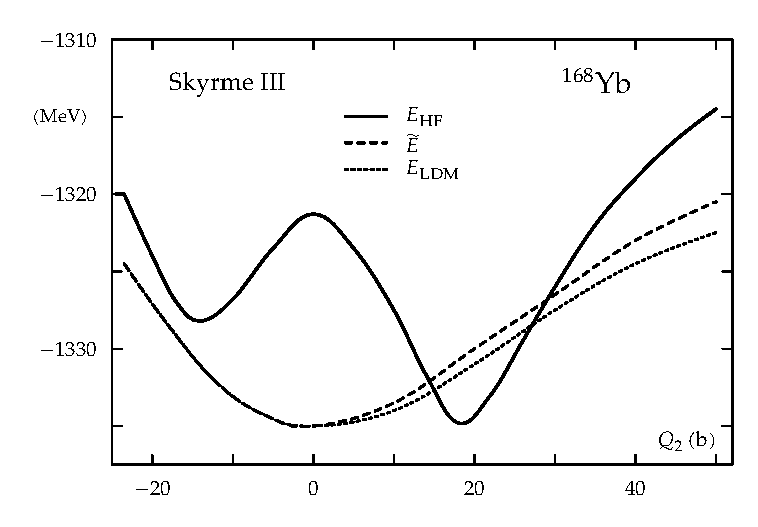
\includegraphics[width=0.75\textwidth]{pictures/2_31}
\par\end{centering}
\caption{\label{fig:2_31}图 2.31 采用 Skyrme III 力计算的 \$\textasciicircum\{168\}}
\end{figure}


\subsection{若干应用}

Strutinsky 壳修正理论在核物理中取得了巨大的成功：
\begin{enumerate}
\item 核质量与结合能：结合液滴模型与 Nilsson 势壳修正，极为成功地再现了全核素区核质量系统学（图 2.32 \cite{NTT69}），尤其精准再现了双幻核
$\ce{^{208}Pb}$ 附近的结合能剧烈振荡结构。
\end{enumerate}
\begin{figure}[H]
\begin{centering}
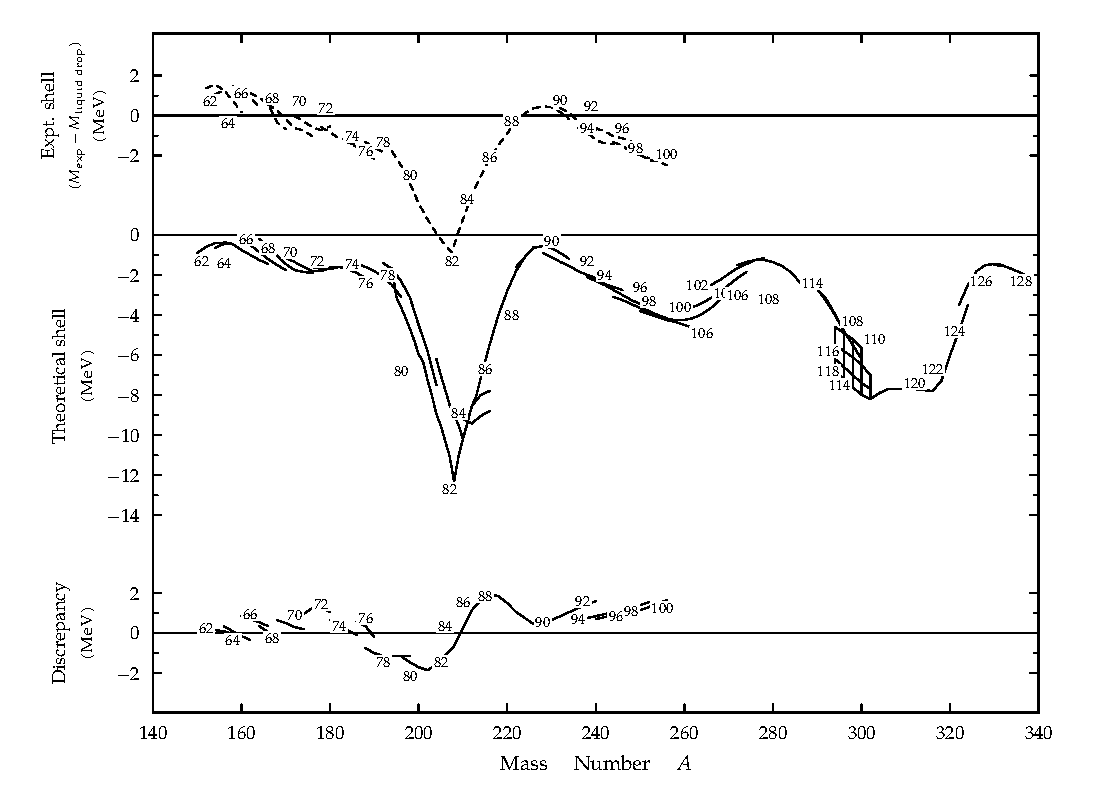
\includegraphics[width=0.75\textwidth]{pictures/2_32}
\par\end{centering}
\caption{\label{fig:2_32}图 2.32 理论计算的质量修正与全核素区实验值的比较（引自 {[}NTT 69{]}）。}
\end{figure}

\begin{enumerate}
\item 多维形变能曲面与双峰裂变势垒：不仅考虑四极形变，还将八极形变、十六极形变等纳入考虑，构建多维形变能曲面。在锕系核中成功预言了双峰裂变势垒（Double-humped
fission barrier），并解释了处于第二极小势阱中的形变同质异能态（裂变同质异能素，fission isomers）。
\item 裂变半衰期与超重核稳定性：通过在多维势能曲面上寻找跨越最低势垒的动力学路径，定量计算重核与超重核的自发裂变寿命，奠定了现代超重核稳定岛（Island
of Stability）预言的理论基石 \cite{Ni72,NN74,BN77}。
\end{enumerate}

